% automatically generated document using lt2circuiTikz
\documentclass[tikz,margin={2pt 2pt 2pt 2pt}]{standalone}
\usepackage[compatibility,siunitx,  americanvoltages, americancurrents, europeanresistors, europeaninductors, americanports,%
  straightlabels, fetbodydiode, straightvoltages]{circuitikz}
\usepackage{tikz,amsmath, amssymb,bm,color,pgfkeys,siunitx,ifthen,ulem}
\usepackage{pgfplots}
\pgfplotsset{compat=1.14}
\usetikzlibrary{shapes,arrows}
%\usepackage{agaramondc}					% Adobe Garamond, custom shape
%\renewcommand{\shapedefault}{rtl} % rtl: roman tabular lining

\makeatletter

%% bandstop filter (adapted from highpass)
\pgfcircdeclarebipole{}{\ctikzvalof{bipoles/highpass/width}}{*bandstop}{\ctikzvalof{bipoles/highpass/width}}{\ctikzvalof{bipoles/highpass/width}}{
	\pgf@circ@res@step = \ctikzvalof{bipoles/highpass/width}\pgf@circ@Rlen
	\divide \pgf@circ@res@step by 2
	
	\pgfpathmoveto{\pgfpoint{\pgf@circ@res@left}{\pgf@circ@res@zero}}
	\pgf@circ@res@other = \pgf@circ@res@left
	\advance\pgf@circ@res@other by \pgf@circ@res@step 
	
	\ifpgf@circuit@dashed
	\pgfsetdash{{0.1cm}{0.1cm}}{0cm} 
	\fi	
	
	% draw outer box
	\pgfsetlinewidth{\pgfkeysvalueof{/tikz/circuitikz/bipoles/thickness}\pgfstartlinewidth}
	\pgfpathrectanglecorners{\pgfpoint{\pgf@circ@res@left}{\pgf@circ@res@up}}{\pgfpoint{\pgf@circ@res@right}{\pgf@circ@res@down}}
	\pgfusepath{draw}
	
	\ifpgf@circuit@inputarrow
	{
		\advance \pgf@circ@res@left by -.5\pgfkeysvalueof{/tikz/circuitikz/bipoles/thickness}\pgfstartlinewidth
		\pgftransformshift{\pgfpoint{\pgf@circ@res@left}{0pt}}
		\pgfnode{inputarrow}{tip}{}{pgf@inputarrow}{\pgfusepath{fill}}
	}
	\fi
	
	% rotate inner symbol
	\def\pgfcircmathresult{\expandafter\pgf@circ@stripdecimals\pgf@circ@direction\pgf@nil}
	\ifnum \pgfcircmathresult > 45 \ifnum \pgfcircmathresult < 135
	\pgftransformrotate{270}
	\fi\fi
	\ifnum \pgfcircmathresult > 134 \ifnum \pgfcircmathresult < 225  % 134 degree, because >= 135 is not possible
	\pgftransformrotate{180}
	\fi\fi
	\ifnum \pgfcircmathresult > 224 \ifnum \pgfcircmathresult < 315
	\pgftransformrotate{90}
	\fi\fi
	
	% draw inner symbol
	\pgfsetdash{}{0pt}	% always draw solid line for inner symbol
	\pgfsetarrows{-} %never draw arrows
	\pgfsetlinewidth{\pgfstartlinewidth}
	\pgfpathmoveto{\pgfpoint{-0.5\pgf@circ@res@step}{0.5\pgf@circ@res@step}}
	\pgfpathsine{\pgfpoint{.25\pgf@circ@res@step}{.25\pgf@circ@res@step}}
	\pgfpathcosine{\pgfpoint{.25\pgf@circ@res@step}{-.25\pgf@circ@res@step}}
	\pgfpathsine{\pgfpoint{.25\pgf@circ@res@step}{-.25\pgf@circ@res@step}}
	\pgfpathcosine{\pgfpoint{.25\pgf@circ@res@step}{.25\pgf@circ@res@step}}
	\pgfusepath{draw}
	
	\pgfpathmoveto{\pgfpoint{-0.5\pgf@circ@res@step}{0}}
	\pgfpathsine{\pgfpoint{.25\pgf@circ@res@step}{.25\pgf@circ@res@step}}
	\pgfpathcosine{\pgfpoint{.25\pgf@circ@res@step}{-.25\pgf@circ@res@step}}
	\pgfpathsine{\pgfpoint{.25\pgf@circ@res@step}{-.25\pgf@circ@res@step}}
	\pgfpathcosine{\pgfpoint{.25\pgf@circ@res@step}{.25\pgf@circ@res@step}}
	\pgfusepath{draw}
	\pgfpathmoveto{\pgfpoint{-0.15\pgf@circ@res@step}{-0.15\pgf@circ@res@step}}
	\pgfpathlineto{\pgfpoint{0.15\pgf@circ@res@step}{0.15\pgf@circ@res@step}}
	\pgfusepath{draw}
	
	\pgfpathmoveto{\pgfpoint{-0.5\pgf@circ@res@step}{-0.5\pgf@circ@res@step}}
	\pgfpathsine{\pgfpoint{.25\pgf@circ@res@step}{.25\pgf@circ@res@step}}
	\pgfpathcosine{\pgfpoint{.25\pgf@circ@res@step}{-.25\pgf@circ@res@step}}
	\pgfpathsine{\pgfpoint{.25\pgf@circ@res@step}{-.25\pgf@circ@res@step}}
	\pgfpathcosine{\pgfpoint{.25\pgf@circ@res@step}{.25\pgf@circ@res@step}}
	\pgfusepath{draw}
	%	\pgfpathmoveto{\pgfpoint{-0.15\pgf@circ@res@step}{-0.65\pgf@circ@res@step}}
	%	\pgfpathlineto{\pgfpoint{0.15\pgf@circ@res@step}{-0.35\pgf@circ@res@step}}
	%	\pgfusepath{draw}
}

\tikzset{
	*bandstop/.style={\circuitikzbasekey, /tikz/to path=\pgf@circ@*bandstop@path},
}
\def\pgf@circ@*bandstop@path#1{\pgf@circ@bipole@path{*bandstop}{#1}}




\makeatother

\usetikzlibrary{backgrounds,calc,positioning}

\usetikzlibrary{circuits.ee.IEC}
\usetikzlibrary{arrows}


% sym32a style

\ctikzset{tripoles/mos style/arrows}
\ctikzset{
	/tikz/circuitikz/quadpoles/coupler/width=1,%1.3
	/tikz/circuitikz/quadpoles/coupler/height=0.952,%1.3
	/tikz/circuitikz/quadpoles/coupler2/width=1,%1.3
	/tikz/circuitikz/quadpoles/coupler2/height=0.952,%1.3
	/tikz/circuitikz/quadpoles/transformer/width=1.425,%1.5
	/tikz/circuitikz/quadpoles/transformer/height=1.425,%1.5
	/tikz/circuitikz/quadpoles/transformer core/width=1.425,%1.5
	/tikz/circuitikz/quadpoles/transformer core/height=1.425,%1.5
	/tikz/circuitikz/quadpoles/gyrator/width=1.425,%1.5
	/tikz/circuitikz/quadpoles/gyrator/height=1.425,%1.5
	%/tikz/circuitikz/monopoles/tlinestub/width=0.1875,%0.25 no effect!
	/tikz/circuitikz/tripoles/american and port/height=0.95,%.8
	/tikz/circuitikz/tripoles/american nand port/height=0.95,%.8
	/tikz/circuitikz/tripoles/american or port/height=0.95,%.8
	/tikz/circuitikz/tripoles/american nor port/height=0.95,%.8
	/tikz/circuitikz/tripoles/american xor port/height=0.95,%.8
	/tikz/circuitikz/tripoles/american xnor port/height=0.95,%.8
	/tikz/circuitikz/bipoles/tline/height=0.4,%0.3
%	/tikz/circuitikz/bipoles/tline/width=1.2,%0.8
	/tikz/circuitikz/bipoles/diode/height=0.375,%
	/tikz/circuitikz/bipoles/diode/width=0.375,%
	/tikz/circuitikz/bipoles/varcap/height=0.375,%
	/tikz/circuitikz/bipoles/varcap/width=0.375,%
	/tikz/circuitikz/tripoles/triac/height=1.05,%
	/tikz/circuitikz/tripoles/triac/width=0.952,%
	/tikz/circuitikz/tripoles/thyristor/height=1.05,%
	/tikz/circuitikz/tripoles/thyristor/width=0.952,%
	/tikz/circuitikz/tripoles/op amp/height=0.952,%
	/tikz/circuitikz/tripoles/op amp/width=1.2,%
	/tikz/circuitikz/tripoles/op amp/font=\footnotesize,
	/tikz/circuitikz/tripoles/gm amp/height=0.952,% 1.7
	/tikz/circuitikz/tripoles/gm amp/width=1.2,% 1.4
	%	/tikz/circuitikz/tripoles/gm amp/font=\footnotesize,
	/tikz/circuitikz/tripoles/plain amp/height=0.952,% 1.7
	/tikz/circuitikz/tripoles/plain amp/width=1.2,% 1.4
	/tikz/circuitikz/bipoles/resistor/voltage/straight label distance/.initial=.8,
	/tikz/circuitikz/bipoles/generic/voltage/straight label distance/.initial=.8,
	/tikz/circuitikz/bipoles/inductor/voltage/straight label distance/.initial=.8,
	/tikz/circuitikz/bipoles/fullgeneric/voltage/straight label distance/.initial=.8,
	/tikz/circuitikz/bipoles/capacitor/voltage/straight label distance/.initial=1.0,
	/tikz/circuitikz/bipoles/thickness=1.6,
}
\ctikzset{v/.append style={/tikz/european voltages}}

\definecolor{netlabelcolor}{rgb}{0, 0, 0.25}
\definecolor{lttotitextcolor}{rgb}{0, 0.4, 0.25}
\definecolor{lttotidrawcolor}{rgb}{0.6, 0.6, 0.6}
\definecolor{netcolor}{rgb}{0, 0, 0.5}

\pgfkeys{/lt2ti/netlabel/font/.initial= \small}
\pgfkeys{/lt2ti/text/font/.initial= \small}

\pgfkeys{/lt2ti/Net/.style= {netcolor}}
\tikzstyle{dashdotdotted}=[dash pattern=on 3pt off 2pt on \the\pgflinewidth off 2pt on \the\pgflinewidth off 2pt]

\pgfkeys{/lt2ti/VArrow/.style= {->,>=latex}}
\pgfkeys{/lt2ti/SArrow/.style= {->,>=angle 90}}

\begin{document}%
	%\centering%
		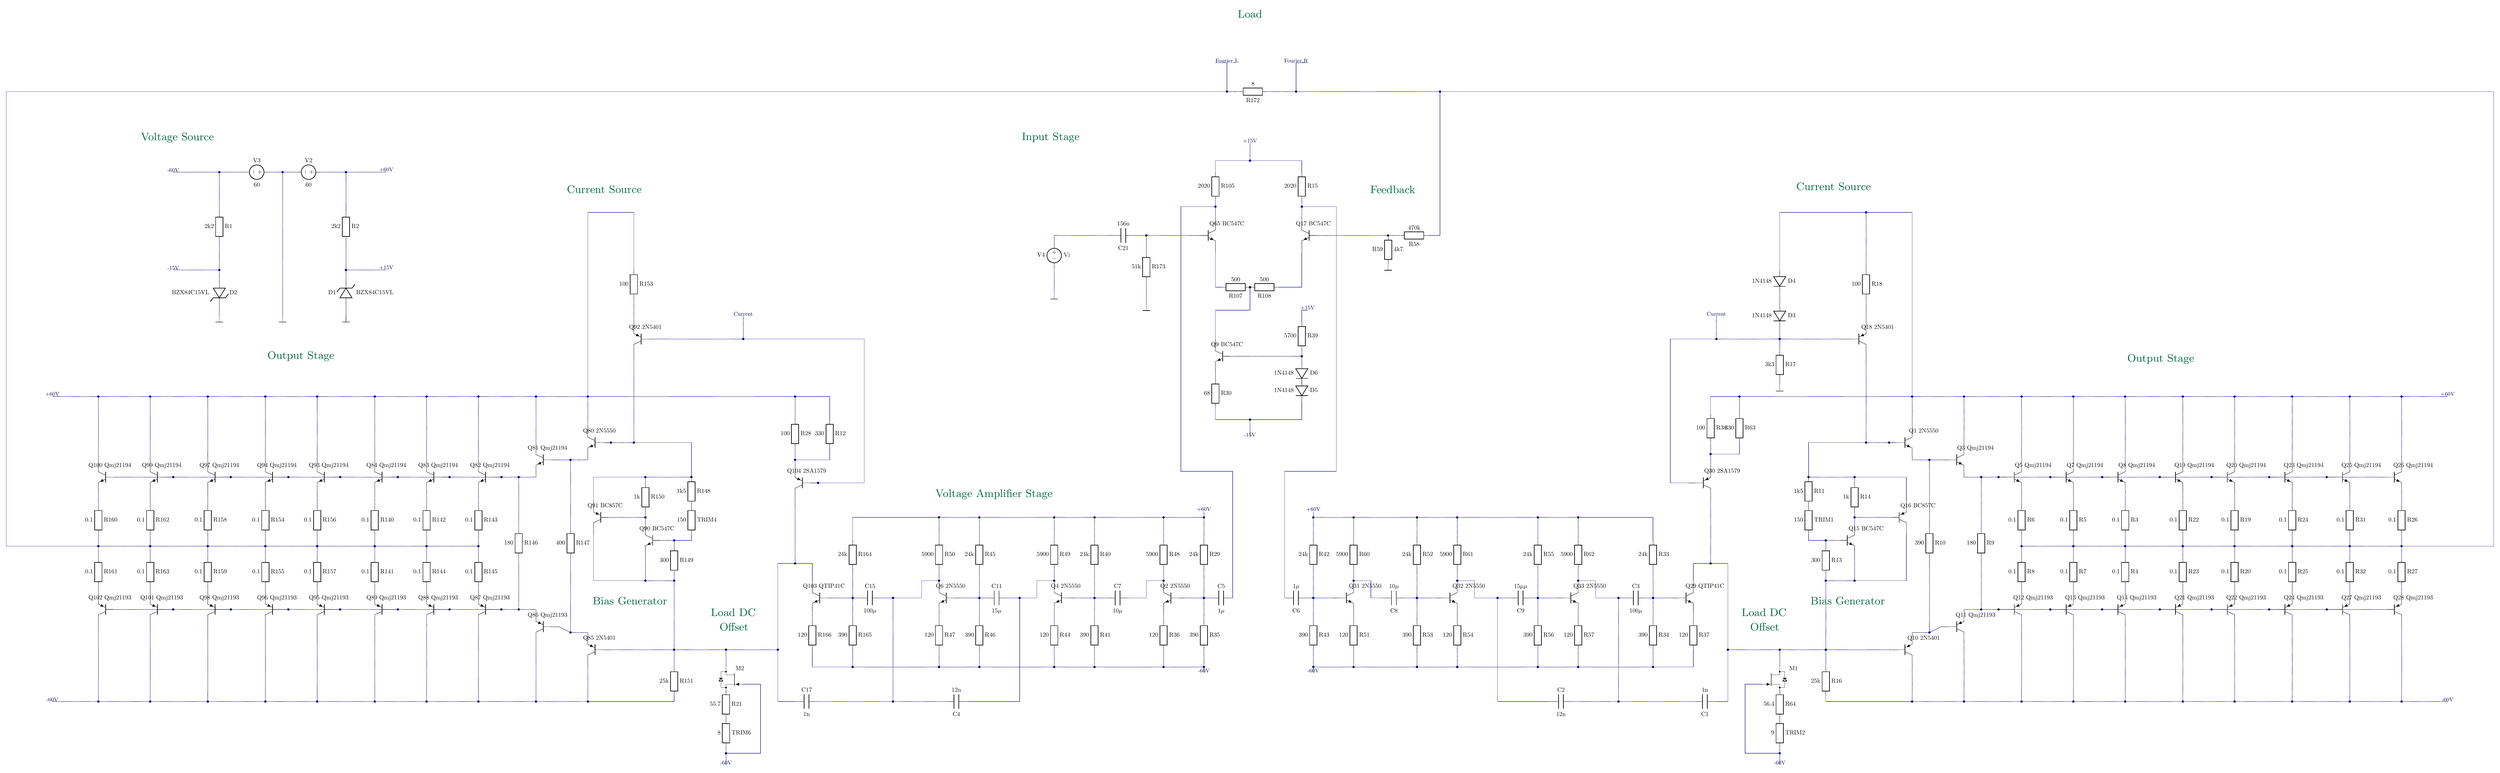
\begin{tikzpicture}[circuit ee IEC, scale=0.6666666667,line width=.5pt]% default: 0.4
	%\tikzstyle{every node}=[font=\small];%
	%\node [draw] at (0.0,0.0) {\pgfkeysvalueof{/tikz/circuitikz/tripoles/op amp/font}};
\draw [/lt2ti/Net](247.5,-129.0)to[*short,-, color=netcolor] (247.5,-129.0);% wire w4_w8 start
\draw [/lt2ti/Net](246.5,-131.5)to[*short,-*, color=netcolor] (246.5,-131.5);% wire w4_w8 end
\draw [/lt2ti/Net](247.5,-129.0) --  (246.5,-129.0) -- (246.5,-131.5); % wire w4_w8 polyline 
\draw [/lt2ti/Net](240.5,-131.5)to[*short,*-, color=netcolor] (240.5,-131.5);% wire w3_w5 start
\draw [/lt2ti/Net](239.5,-129.0)to[*short,-, color=netcolor] (239.5,-129.0);% wire w3_w5 end
\draw [/lt2ti/Net](240.5,-131.5) --  (240.5,-129.0) -- (239.5,-129.0); % wire w3_w5 polyline 
\draw [/lt2ti/Net](241.5,-131.5)to[*short,-*, color=netcolor] (240.5,-131.5);% wire w7
\draw [/lt2ti/Net](246.5,-131.5)to[*short,*-, color=netcolor] (244.0,-131.5);% wire w9
\draw [/lt2ti/Net](259.0,-131.5)to[*short,*-*, color=netcolor] (246.5,-131.5);% wire w10
\draw [/lt2ti/Net](259.0,-131.5)to[*short,*-, color=netcolor] (259.0,-131.5);% wire w39_w40 start
\draw [/lt2ti/Net](258.0,-144.0)to[*short,-, color=netcolor] (258.0,-144.0);% wire w39_w40 end
\draw [/lt2ti/Net](259.0,-131.5) --  (259.0,-144.0) -- (258.0,-144.0); % wire w39_w40 polyline 
\draw [/lt2ti/Net](242.5,-137.5)to[*short,*-, color=netcolor] (242.5,-136.0);% wire w12
\draw [/lt2ti/Net](242.5,-137.5)to[*short,*-, color=netcolor] (242.5,-137.5);% wire w13_w21 start
\draw [/lt2ti/Net](239.5,-138.5)to[*short,-, color=netcolor] (239.5,-138.5);% wire w13_w21 end
\draw [/lt2ti/Net](242.5,-137.5) --  (239.5,-137.5) -- (239.5,-138.5); % wire w13_w21 polyline 
\draw [/lt2ti/Net](153.0,-138.5)to[*short,*-, color=netcolor] (149.0,-138.5);% wire w15
\draw [/lt2ti/Net](155.0,-138.5)to[*short,-*, color=netcolor] (153.0,-138.5);% wire w16
\draw [/lt2ti/Net](158.5,-138.5)to[*short,*-, color=netcolor] (157.5,-138.5);% wire w17
\draw [/lt2ti/Net](159.5,-138.5)to[*short,-*, color=netcolor] (158.5,-138.5);% wire w18
\draw [/lt2ti/Net](164.0,-138.5)to[*short,*-, color=netcolor] (162.0,-138.5);% wire w19
\draw [/lt2ti/Net](167.5,-138.5)to[*short,-*, color=netcolor] (164.0,-138.5);% wire w20
\draw [/lt2ti/Net](247.0,-138.5)to[*short,-, color=netcolor] (247.0,-138.5);% wire w14_w22 start
\draw [/lt2ti/Net](242.5,-137.5)to[*short,-*, color=netcolor] (242.5,-137.5);% wire w14_w22 end
\draw [/lt2ti/Net](247.0,-138.5) --  (247.0,-137.5) -- (242.5,-137.5); % wire w14_w22 polyline 
\draw [/lt2ti/Net](239.5,-141.5)to[*short,*-, color=netcolor] (239.5,-141.0);% wire w23
\draw [/lt2ti/Net](247.0,-141.5)to[*short,*-, color=netcolor] (247.0,-141.0);% wire w25
\draw [/lt2ti/Net](153.0,-142.0)to[*short,-*, color=netcolor] (153.0,-138.5);% wire w27
\draw [/lt2ti/Net](164.0,-142.0)to[*short,-*, color=netcolor] (164.0,-138.5);% wire w28
\draw [/lt2ti/Net](296.0,-142.0)to[*short,*-, color=netcolor] (296.0,-142.0);% wire w30_w48 start
\draw [/lt2ti/Net](288.5,-147.0)to[*short,-, color=netcolor] (288.5,-147.0);% wire w30_w48 end
\draw [/lt2ti/Net](296.0,-142.0) --  (288.5,-142.0) -- (288.5,-147.0); % wire w30_w48 polyline 
\draw [/lt2ti/Net](239.5,-142.5)to[*short,-*, color=netcolor] (239.5,-141.5);% wire w32
\draw [/lt2ti/Net](247.0,-142.5)to[*short,-*, color=netcolor] (247.0,-141.5);% wire w33
\draw [/lt2ti/Net](230.5,-144.0)to[*short,-, color=netcolor] (225.5,-144.0);% wire w34
\draw [/lt2ti/Net](233.5,-144.0)to[*short,*-, color=netcolor] (232.5,-144.0);% wire w35
\draw [/lt2ti/Net](237.5,-144.0)to[*short,-*, color=netcolor] (233.5,-144.0);% wire w36
\draw [/lt2ti/Net](254.5,-144.0)to[*short,*-, color=netcolor] (249.0,-144.0);% wire w37
\draw [/lt2ti/Net](255.5,-144.0)to[*short,-*, color=netcolor] (254.5,-144.0);% wire w38
\draw [/lt2ti/Net](225.5,-144.5)to[*short,-, color=netcolor] (225.5,-144.0);% wire w41
\draw [/lt2ti/Net](233.5,-145.5)to[*short,-*, color=netcolor] (233.5,-144.0);% wire w42
\draw [/lt2ti/Net](153.0,-147.0)to[*short,*-, color=netcolor] (153.0,-144.5);% wire w43
\draw [/lt2ti/Net](153.0,-147.0)to[*short,*-, color=netcolor] (149.0,-147.0);% wire w44
\draw [/lt2ti/Net](164.0,-147.0)to[*short,*-, color=netcolor] (164.0,-144.5);% wire w45
\draw [/lt2ti/Net](167.5,-147.0)to[*short,-*, color=netcolor] (164.0,-147.0);% wire w46
\draw [/lt2ti/Net](296.0,-147.0)to[*short,-*, color=netcolor] (296.0,-142.0);% wire w49
\draw [/lt2ti/Net](153.0,-148.0)to[*short,-*, color=netcolor] (153.0,-147.0);% wire w50
\draw [/lt2ti/Net](164.0,-148.0)to[*short,-*, color=netcolor] (164.0,-147.0);% wire w51
\draw [/lt2ti/Net](240.0,-148.5)to[*short,-, color=netcolor] (240.0,-148.5);% wire w52_w53 start
\draw [/lt2ti/Net](239.5,-145.5)to[*short,-, color=netcolor] (239.5,-145.5);% wire w52_w53 end
\draw [/lt2ti/Net](240.0,-148.5) --  (239.5,-148.5) -- (239.5,-145.5); % wire w52_w53 polyline 
\draw [/lt2ti/Net](247.0,-145.5)to[*short,-, color=netcolor] (247.0,-145.5);% wire w54_w55 start
\draw [/lt2ti/Net](245.0,-148.5)to[*short,-, color=netcolor] (245.0,-148.5);% wire w54_w55 end
\draw [/lt2ti/Net](247.0,-145.5) --  (247.0,-148.5) -- (245.0,-148.5); % wire w54_w55 polyline 
\draw [/lt2ti/Net](225.5,-149.0)to[*short,-, color=netcolor] (225.5,-147.0);% wire w56
\draw [/lt2ti/Net](233.5,-150.0)to[*short,-, color=netcolor] (233.5,-148.0);% wire w57
\draw [/lt2ti/Net](288.5,-150.0)to[*short,-, color=netcolor] (288.5,-149.0);% wire w58
\draw [/lt2ti/Net](247.5,-150.5)to[*short,-, color=netcolor] (247.5,-150.5);% wire w61_w66 start
\draw [/lt2ti/Net](247.0,-151.5)to[*short,-, color=netcolor] (247.0,-151.5);% wire w61_w66 end
\draw [/lt2ti/Net](247.5,-150.5) --  (247.0,-150.5) -- (247.0,-151.5); % wire w61_w66 polyline 
\draw [/lt2ti/Net](153.0,-151.0)to[*short,-, color=netcolor] (153.0,-150.0);% wire w62
\draw [/lt2ti/Net](158.5,-151.0)to[*short,-*, color=netcolor] (158.5,-138.5);% wire w63
\draw [/lt2ti/Net](164.0,-151.0)to[*short,-, color=netcolor] (164.0,-150.0);% wire w64
\draw [/lt2ti/Net](189.0,-151.5)to[*short,-, color=netcolor] (189.0,-149.5);% wire w65
\draw [/lt2ti/Net](296.0,-151.5)to[*short,-, color=netcolor] (296.0,-149.5);% wire w67
\draw [/lt2ti/Net](198.5,-153.0)to[*short,*-, color=netcolor] (198.5,-151.0);% wire w68
\draw [/lt2ti/Net](198.5,-153.0)to[*short,*-, color=netcolor] (191.0,-153.0);% wire w69
\draw [/lt2ti/Net](239.5,-153.0)to[*short,-, color=netcolor] (239.5,-153.0);% wire w71_w59_w60 start
\draw [/lt2ti/Net](242.5,-148.5)to[*short,-*, color=netcolor] (242.5,-148.5);% wire w71_w59_w60 end
\draw [/lt2ti/Net](239.5,-153.0) --  (239.5,-150.5) --  (242.5,-150.5) -- (242.5,-148.5); % wire w71_w59_w60 polyline 
\draw [/lt2ti/Net](283.0,-153.0)to[*short,*-, color=netcolor] (283.0,-151.0);% wire w72
\draw [/lt2ti/Net](288.5,-153.0)to[*short,*-, color=netcolor] (288.5,-152.0);% wire w74
\draw [/lt2ti/Net](288.5,-153.0)to[*short,*-*, color=netcolor] (283.0,-153.0);% wire w75
\draw [/lt2ti/Net](294.0,-153.0)to[*short,-*, color=netcolor] (288.5,-153.0);% wire w76
\draw [/lt2ti/Net](288.5,-154.0)to[*short,-*, color=netcolor] (288.5,-153.0);% wire w77
\draw [/lt2ti/Net](247.0,-154.5)to[*short,*-, color=netcolor] (247.0,-154.0);% wire w78
\draw [/lt2ti/Net](247.0,-154.5)to[*short,*-, color=netcolor] (241.5,-154.5);% wire w79
\draw [/lt2ti/Net](247.0,-155.0)to[*short,-*, color=netcolor] (247.0,-154.5);% wire w80
\draw [/lt2ti/Net](239.5,-156.5)to[*short,-, color=netcolor] (239.5,-156.0);% wire w81
\draw [/lt2ti/Net](247.0,-157.0)to[*short,-, color=netcolor] (247.0,-156.5);% wire w82
\draw [/lt2ti/Net](288.5,-157.0)to[*short,-, color=netcolor] (288.5,-156.5);% wire w83
\draw [/lt2ti/Net](142.5,-158.0)to[*short,*-, color=netcolor] (138.5,-158.0);% wire w84
\draw [/lt2ti/Net](147.0,-158.0)to[*short,*-*, color=netcolor] (142.5,-158.0);% wire w85
\draw [/lt2ti/Net](152.0,-158.0)to[*short,*-*, color=netcolor] (147.0,-158.0);% wire w86
\draw [/lt2ti/Net](157.0,-158.0)to[*short,*-*, color=netcolor] (152.0,-158.0);% wire w87
\draw [/lt2ti/Net](161.5,-158.0)to[*short,*-*, color=netcolor] (157.0,-158.0);% wire w88
\draw [/lt2ti/Net](166.5,-158.0)to[*short,*-*, color=netcolor] (161.5,-158.0);% wire w89
\draw [/lt2ti/Net](171.0,-158.0)to[*short,*-*, color=netcolor] (166.5,-158.0);% wire w90
\draw [/lt2ti/Net](175.5,-158.0)to[*short,*-*, color=netcolor] (171.0,-158.0);% wire w91
\draw [/lt2ti/Net](180.5,-158.0)to[*short,*-*, color=netcolor] (175.5,-158.0);% wire w92
\draw [/lt2ti/Net](185.0,-158.0)to[*short,*-*, color=netcolor] (180.5,-158.0);% wire w94
\draw [/lt2ti/Net](185.0,-158.0)to[*short,*-, color=netcolor] (185.0,-158.0);% wire w93_w29_w47 start
\draw [/lt2ti/Net](189.0,-147.0)to[*short,-, color=netcolor] (189.0,-147.0);% wire w93_w29_w47 end
\draw [/lt2ti/Net](185.0,-158.0) --  (185.0,-142.0) --  (189.0,-142.0) -- (189.0,-147.0); % wire w93_w29_w47 polyline 
\draw [/lt2ti/Net](203.0,-158.0)to[*short,*-*, color=netcolor] (185.0,-158.0);% wire w95
\draw [/lt2ti/Net](285.0,-158.0)to[*short,*-, color=netcolor] (285.0,-158.0);% wire w97_w110 start
\draw [/lt2ti/Net](282.5,-159.5)to[*short,-, color=netcolor] (282.5,-159.5);% wire w97_w110 end
\draw [/lt2ti/Net](285.0,-158.0) --  (282.5,-158.0) -- (282.5,-159.5); % wire w97_w110 polyline 
\draw [/lt2ti/Net](300.0,-158.0)to[*short,*-*, color=netcolor] (285.0,-158.0);% wire w99
\draw [/lt2ti/Net](300.0,-158.0)to[*short,*-, color=netcolor] (300.0,-158.0);% wire w31_w98 start
\draw [/lt2ti/Net](296.0,-142.0)to[*short,-*, color=netcolor] (296.0,-142.0);% wire w31_w98 end
\draw [/lt2ti/Net](300.0,-158.0) --  (300.0,-142.0) -- (296.0,-142.0); % wire w31_w98 polyline 
\draw [/lt2ti/Net](304.5,-158.0)to[*short,*-*, color=netcolor] (300.0,-158.0);% wire w100
\draw [/lt2ti/Net](309.5,-158.0)to[*short,*-*, color=netcolor] (304.5,-158.0);% wire w101
\draw [/lt2ti/Net](314.0,-158.0)to[*short,*-*, color=netcolor] (309.5,-158.0);% wire w102
\draw [/lt2ti/Net](318.5,-158.0)to[*short,*-*, color=netcolor] (314.0,-158.0);% wire w103
\draw [/lt2ti/Net](323.5,-158.0)to[*short,*-*, color=netcolor] (318.5,-158.0);% wire w104
\draw [/lt2ti/Net](328.0,-158.0)to[*short,*-*, color=netcolor] (323.5,-158.0);% wire w105
\draw [/lt2ti/Net](333.0,-158.0)to[*short,*-*, color=netcolor] (328.0,-158.0);% wire w106
\draw [/lt2ti/Net](338.0,-158.0)to[*short,*-*, color=netcolor] (333.0,-158.0);% wire w107
\draw [/lt2ti/Net](342.5,-158.0)to[*short,*-*, color=netcolor] (338.0,-158.0);% wire w108
\draw [/lt2ti/Net](346.5,-158.0)to[*short,-*, color=netcolor] (342.5,-158.0);% wire w109
\draw [/lt2ti/Net](285.0,-159.5)to[*short,-*, color=netcolor] (285.0,-158.0);% wire w111
\draw [/lt2ti/Net](203.0,-160.0)to[*short,-*, color=netcolor] (203.0,-158.0);% wire w112
\draw [/lt2ti/Net](206.0,-160.0)to[*short,-, color=netcolor] (206.0,-160.0);% wire w96_w113 start
\draw [/lt2ti/Net](203.0,-158.0)to[*short,-*, color=netcolor] (203.0,-158.0);% wire w96_w113 end
\draw [/lt2ti/Net](206.0,-160.0) --  (206.0,-158.0) -- (203.0,-158.0); % wire w96_w113 polyline 
\draw [/lt2ti/Net](242.5,-160.0)to[*short,*-, color=netcolor] (242.5,-160.0);% wire w114_w115 start
\draw [/lt2ti/Net](239.5,-159.0)to[*short,-, color=netcolor] (239.5,-159.0);% wire w114_w115 end
\draw [/lt2ti/Net](242.5,-160.0) --  (239.5,-160.0) -- (239.5,-159.0); % wire w114_w115 polyline 
\draw [/lt2ti/Net](247.0,-158.5)to[*short,-, color=netcolor] (247.0,-158.5);% wire w116_w117 start
\draw [/lt2ti/Net](242.5,-160.0)to[*short,-*, color=netcolor] (242.5,-160.0);% wire w116_w117 end
\draw [/lt2ti/Net](247.0,-158.5) --  (247.0,-160.0) -- (242.5,-160.0); % wire w116_w117 polyline 
\draw [/lt2ti/Net](185.0,-160.5)to[*short,-*, color=netcolor] (185.0,-158.0);% wire w118
\draw [/lt2ti/Net](300.0,-160.5)to[*short,-*, color=netcolor] (300.0,-158.0);% wire w119
\draw [/lt2ti/Net](242.5,-161.5)to[*short,-*, color=netcolor] (242.5,-160.0);% wire w120
\draw [/lt2ti/Net](180.5,-162.0)to[*short,-*, color=netcolor] (180.5,-158.0);% wire w121
\draw [/lt2ti/Net](187.0,-162.0)to[*short,*-, color=netcolor] (186.5,-162.0);% wire w122
\draw [/lt2ti/Net](189.0,-162.0)to[*short,*-, color=netcolor] (189.0,-154.5);% wire w123
\draw [/lt2ti/Net](189.0,-162.0)to[*short,*-*, color=netcolor] (187.0,-162.0);% wire w124
\draw [/lt2ti/Net](296.0,-162.0)to[*short,*-, color=netcolor] (296.0,-154.5);% wire w126
\draw [/lt2ti/Net](296.0,-162.0)to[*short,*-, color=netcolor] (296.0,-162.0);% wire w127_w175 start
\draw [/lt2ti/Net](291.0,-165.0)to[*short,-*, color=netcolor] (291.0,-165.0);% wire w127_w175 end
\draw [/lt2ti/Net](296.0,-162.0) --  (291.0,-162.0) -- (291.0,-165.0); % wire w127_w175 polyline 
\draw [/lt2ti/Net](298.0,-162.0)to[*short,*-*, color=netcolor] (296.0,-162.0);% wire w128
\draw [/lt2ti/Net](298.5,-162.0)to[*short,-*, color=netcolor] (298.0,-162.0);% wire w129
\draw [/lt2ti/Net](304.5,-162.0)to[*short,-*, color=netcolor] (304.5,-158.0);% wire w130
\draw [/lt2ti/Net](282.5,-163.0)to[*short,*-, color=netcolor] (282.5,-162.0);% wire w131
\draw [/lt2ti/Net](285.0,-162.0)to[*short,-, color=netcolor] (285.0,-162.0);% wire w132_w133 start
\draw [/lt2ti/Net](282.5,-163.0)to[*short,-*, color=netcolor] (282.5,-163.0);% wire w132_w133 end
\draw [/lt2ti/Net](285.0,-162.0) --  (285.0,-163.0) -- (282.5,-163.0); % wire w132_w133 polyline 
\draw [/lt2ti/Net](142.5,-163.5)to[*short,-*, color=netcolor] (142.5,-158.0);% wire w134
\draw [/lt2ti/Net](147.0,-163.5)to[*short,-*, color=netcolor] (147.0,-158.0);% wire w135
\draw [/lt2ti/Net](152.0,-163.5)to[*short,-*, color=netcolor] (152.0,-158.0);% wire w136
\draw [/lt2ti/Net](157.0,-163.5)to[*short,-*, color=netcolor] (157.0,-158.0);% wire w137
\draw [/lt2ti/Net](161.5,-163.5)to[*short,-*, color=netcolor] (161.5,-158.0);% wire w138
\draw [/lt2ti/Net](166.5,-163.5)to[*short,-*, color=netcolor] (166.5,-158.0);% wire w139
\draw [/lt2ti/Net](171.0,-163.5)to[*short,-*, color=netcolor] (171.0,-158.0);% wire w140
\draw [/lt2ti/Net](175.5,-163.5)to[*short,-*, color=netcolor] (175.5,-158.0);% wire w141
\draw [/lt2ti/Net](183.5,-163.5)to[*short,*-, color=netcolor] (182.5,-163.5);% wire w142
\draw [/lt2ti/Net](185.0,-163.5)to[*short,-*, color=netcolor] (183.5,-163.5);% wire w143
\draw [/lt2ti/Net](203.0,-163.5)to[*short,*-, color=netcolor] (203.0,-162.5);% wire w144
\draw [/lt2ti/Net](206.0,-162.5)to[*short,-, color=netcolor] (206.0,-162.5);% wire w145_w146 start
\draw [/lt2ti/Net](203.0,-163.5)to[*short,-*, color=netcolor] (203.0,-163.5);% wire w145_w146 end
\draw [/lt2ti/Net](206.0,-162.5) --  (206.0,-163.5) -- (203.0,-163.5); % wire w145_w146 polyline 
\draw [/lt2ti/Net](301.5,-163.5)to[*short,*-, color=netcolor] (300.0,-163.5);% wire w147
\draw [/lt2ti/Net](302.5,-163.5)to[*short,-*, color=netcolor] (301.5,-163.5);% wire w148
\draw [/lt2ti/Net](309.5,-163.5)to[*short,-*, color=netcolor] (309.5,-158.0);% wire w149
\draw [/lt2ti/Net](314.0,-163.5)to[*short,-*, color=netcolor] (314.0,-158.0);% wire w150
\draw [/lt2ti/Net](318.5,-163.5)to[*short,-*, color=netcolor] (318.5,-158.0);% wire w151
\draw [/lt2ti/Net](323.5,-163.5)to[*short,-*, color=netcolor] (323.5,-158.0);% wire w152
\draw [/lt2ti/Net](328.0,-163.5)to[*short,-*, color=netcolor] (328.0,-158.0);% wire w153
\draw [/lt2ti/Net](333.0,-163.5)to[*short,-*, color=netcolor] (333.0,-158.0);% wire w154
\draw [/lt2ti/Net](338.0,-163.5)to[*short,-*, color=netcolor] (338.0,-158.0);% wire w155
\draw [/lt2ti/Net](342.5,-163.5)to[*short,-*, color=netcolor] (342.5,-158.0);% wire w156
\draw [/lt2ti/Net](203.0,-164.0)to[*short,-*, color=netcolor] (203.0,-163.5);% wire w157
\draw [/lt2ti/Net](282.5,-164.0)to[*short,-*, color=netcolor] (282.5,-163.0);% wire w158
\draw [/lt2ti/Net](149.0,-165.0)to[*short,*-, color=netcolor] (144.5,-165.0);% wire w163
\draw [/lt2ti/Net](154.0,-165.0)to[*short,*-*, color=netcolor] (149.0,-165.0);% wire w164
\draw [/lt2ti/Net](159.0,-165.0)to[*short,*-*, color=netcolor] (154.0,-165.0);% wire w165
\draw [/lt2ti/Net](163.5,-165.0)to[*short,*-*, color=netcolor] (159.0,-165.0);% wire w166
\draw [/lt2ti/Net](168.5,-165.0)to[*short,*-*, color=netcolor] (163.5,-165.0);% wire w167
\draw [/lt2ti/Net](173.0,-165.0)to[*short,*-*, color=netcolor] (168.5,-165.0);% wire w168
\draw [/lt2ti/Net](177.5,-165.0)to[*short,*-*, color=netcolor] (173.0,-165.0);% wire w169
\draw [/lt2ti/Net](179.0,-165.0)to[*short,*-*, color=netcolor] (177.5,-165.0);% wire w170
\draw [/lt2ti/Net](180.5,-165.0)to[*short,-*, color=netcolor] (179.0,-165.0);% wire w171
\draw [/lt2ti/Net](190.0,-165.0)to[*short,*-, color=netcolor] (190.0,-165.0);% wire w172_w194 start
\draw [/lt2ti/Net](185.5,-167.0)to[*short,-, color=netcolor] (185.5,-167.0);% wire w172_w194 end
\draw [/lt2ti/Net](190.0,-165.0) --  (185.5,-165.0) -- (185.5,-167.0); % wire w172_w194 polyline 
\draw [/lt2ti/Net](194.0,-165.0)to[*short,*-*, color=netcolor] (190.0,-165.0);% wire w174
\draw [/lt2ti/Net](194.0,-165.0)to[*short,*-, color=netcolor] (194.0,-165.0);% wire w125_w173 start
\draw [/lt2ti/Net](189.0,-162.0)to[*short,-*, color=netcolor] (189.0,-162.0);% wire w125_w173 end
\draw [/lt2ti/Net](194.0,-165.0) --  (194.0,-162.0) -- (189.0,-162.0); % wire w125_w173 polyline 
\draw [/lt2ti/Net](295.0,-165.0)to[*short,*-*, color=netcolor] (291.0,-165.0);% wire w176
\draw [/lt2ti/Net](306.0,-165.0)to[*short,*-, color=netcolor] (304.5,-165.0);% wire w178
\draw [/lt2ti/Net](307.5,-165.0)to[*short,*-*, color=netcolor] (306.0,-165.0);% wire w179
\draw [/lt2ti/Net](312.0,-165.0)to[*short,*-*, color=netcolor] (307.5,-165.0);% wire w180
\draw [/lt2ti/Net](316.5,-165.0)to[*short,*-*, color=netcolor] (312.0,-165.0);% wire w181
\draw [/lt2ti/Net](321.5,-165.0)to[*short,*-*, color=netcolor] (316.5,-165.0);% wire w182
\draw [/lt2ti/Net](326.0,-165.0)to[*short,*-*, color=netcolor] (321.5,-165.0);% wire w183
\draw [/lt2ti/Net](331.0,-165.0)to[*short,*-*, color=netcolor] (326.0,-165.0);% wire w184
\draw [/lt2ti/Net](336.0,-165.0)to[*short,*-*, color=netcolor] (331.0,-165.0);% wire w185
\draw [/lt2ti/Net](340.5,-165.0)to[*short,-*, color=netcolor] (336.0,-165.0);% wire w186
\draw [/lt2ti/Net](190.0,-165.5)to[*short,-*, color=netcolor] (190.0,-165.0);% wire w187
\draw [/lt2ti/Net](205.0,-165.5)to[*short,*-, color=netcolor] (204.5,-165.5);% wire w188
\draw [/lt2ti/Net](205.0,-165.5)to[*short,*-, color=netcolor] (205.0,-165.5);% wire w190_w70_w189 start
\draw [/lt2ti/Net](198.5,-153.0)to[*short,-*, color=netcolor] (198.5,-153.0);% wire w190_w70_w189 end
\draw [/lt2ti/Net](205.0,-165.5) --  (209.0,-165.5) --  (209.0,-153.0) -- (198.5,-153.0); % wire w190_w70_w189 polyline 
\draw [/lt2ti/Net](280.5,-165.5)to[*short,-, color=netcolor] (280.5,-165.5);% wire w192_w73_w191 start
\draw [/lt2ti/Net](283.0,-153.0)to[*short,-*, color=netcolor] (283.0,-153.0);% wire w192_w73_w191 end
\draw [/lt2ti/Net](280.5,-165.5) --  (279.0,-165.5) --  (279.0,-153.0) -- (283.0,-153.0); % wire w192_w73_w191 polyline 
\draw [/lt2ti/Net](295.0,-165.5)to[*short,-*, color=netcolor] (295.0,-165.0);% wire w193
\draw [/lt2ti/Net](299.5,-167.0)to[*short,-, color=netcolor] (299.5,-167.0);% wire w177_w195 start
\draw [/lt2ti/Net](295.0,-165.0)to[*short,-*, color=netcolor] (295.0,-165.0);% wire w177_w195 end
\draw [/lt2ti/Net](299.5,-167.0) --  (299.5,-165.0) -- (295.0,-165.0); % wire w177_w195 polyline 
\draw [/lt2ti/Net](142.5,-167.5)to[*short,-, color=netcolor] (142.5,-166.5);% wire w196
\draw [/lt2ti/Net](147.0,-167.5)to[*short,-, color=netcolor] (147.0,-166.5);% wire w197
\draw [/lt2ti/Net](152.0,-167.5)to[*short,-, color=netcolor] (152.0,-166.5);% wire w198
\draw [/lt2ti/Net](157.0,-167.5)to[*short,-, color=netcolor] (157.0,-166.5);% wire w199
\draw [/lt2ti/Net](161.5,-167.5)to[*short,-, color=netcolor] (161.5,-166.5);% wire w200
\draw [/lt2ti/Net](166.5,-167.5)to[*short,-, color=netcolor] (166.5,-166.5);% wire w201
\draw [/lt2ti/Net](171.0,-167.5)to[*short,-, color=netcolor] (171.0,-166.5);% wire w202
\draw [/lt2ti/Net](175.5,-167.5)to[*short,-, color=netcolor] (175.5,-166.5);% wire w203
\draw [/lt2ti/Net](309.5,-167.5)to[*short,-, color=netcolor] (309.5,-166.5);% wire w204
\draw [/lt2ti/Net](314.0,-167.5)to[*short,-, color=netcolor] (314.0,-166.5);% wire w205
\draw [/lt2ti/Net](318.5,-167.5)to[*short,-, color=netcolor] (318.5,-166.5);% wire w206
\draw [/lt2ti/Net](323.5,-167.5)to[*short,-, color=netcolor] (323.5,-166.5);% wire w207
\draw [/lt2ti/Net](328.0,-167.5)to[*short,-, color=netcolor] (328.0,-166.5);% wire w208
\draw [/lt2ti/Net](333.0,-167.5)to[*short,-, color=netcolor] (333.0,-166.5);% wire w209
\draw [/lt2ti/Net](338.0,-167.5)to[*short,-, color=netcolor] (338.0,-166.5);% wire w210
\draw [/lt2ti/Net](342.5,-167.5)to[*short,-, color=netcolor] (342.5,-166.5);% wire w211
\draw [/lt2ti/Net](190.0,-168.5)to[*short,*-, color=netcolor] (190.0,-168.0);% wire w212
\draw [/lt2ti/Net](190.0,-168.5)to[*short,*-, color=netcolor] (187.5,-168.5);% wire w213
\draw [/lt2ti/Net](215.5,-168.5)to[*short,*-, color=netcolor] (215.5,-168.5);% wire w214_w239 start
\draw [/lt2ti/Net](208.0,-170.5)to[*short,-, color=netcolor] (208.0,-170.5);% wire w214_w239 end
\draw [/lt2ti/Net](215.5,-168.5) --  (208.0,-168.5) -- (208.0,-170.5); % wire w214_w239 polyline 
\draw [/lt2ti/Net](219.0,-168.5)to[*short,*-*, color=netcolor] (215.5,-168.5);% wire w215
\draw [/lt2ti/Net](225.5,-168.5)to[*short,*-*, color=netcolor] (219.0,-168.5);% wire w216
\draw [/lt2ti/Net](229.0,-168.5)to[*short,*-*, color=netcolor] (225.5,-168.5);% wire w217
\draw [/lt2ti/Net](235.0,-168.5)to[*short,*-*, color=netcolor] (229.0,-168.5);% wire w218
\draw [/lt2ti/Net](238.5,-168.5)to[*short,*-, color=netcolor] (238.5,-168.0);% wire w219
\draw [/lt2ti/Net](238.5,-168.5)to[*short,*-*, color=netcolor] (235.0,-168.5);% wire w220
\draw [/lt2ti/Net](248.0,-168.5)to[*short,*-, color=netcolor] (248.0,-168.0);% wire w221
\draw [/lt2ti/Net](251.5,-168.5)to[*short,*-*, color=netcolor] (248.0,-168.5);% wire w222
\draw [/lt2ti/Net](257.0,-168.5)to[*short,*-*, color=netcolor] (251.5,-168.5);% wire w223
\draw [/lt2ti/Net](260.5,-168.5)to[*short,*-*, color=netcolor] (257.0,-168.5);% wire w224
\draw [/lt2ti/Net](267.5,-168.5)to[*short,*-*, color=netcolor] (260.5,-168.5);% wire w225
\draw [/lt2ti/Net](271.0,-168.5)to[*short,*-*, color=netcolor] (267.5,-168.5);% wire w226
\draw [/lt2ti/Net](295.0,-168.5)to[*short,*-, color=netcolor] (295.0,-168.0);% wire w228
\draw [/lt2ti/Net](297.5,-168.5)to[*short,-*, color=netcolor] (295.0,-168.5);% wire w229
\draw [/lt2ti/Net](190.0,-169.0)to[*short,-*, color=netcolor] (190.0,-168.5);% wire w230
\draw [/lt2ti/Net](295.0,-169.0)to[*short,-*, color=netcolor] (295.0,-168.5);% wire w231
\draw [/lt2ti/Net](179.0,-169.5)to[*short,-*, color=netcolor] (179.0,-165.0);% wire w232
\draw [/lt2ti/Net](183.5,-169.5)to[*short,-*, color=netcolor] (183.5,-163.5);% wire w233
\draw [/lt2ti/Net](301.5,-169.5)to[*short,-*, color=netcolor] (301.5,-163.5);% wire w234
\draw [/lt2ti/Net](306.0,-169.5)to[*short,-*, color=netcolor] (306.0,-165.0);% wire w235
\draw [/lt2ti/Net](192.5,-170.5)to[*short,*-, color=netcolor] (192.0,-170.5);% wire w236
\draw [/lt2ti/Net](194.0,-170.0)to[*short,-, color=netcolor] (194.0,-170.0);% wire w237_w238 start
\draw [/lt2ti/Net](192.5,-170.5)to[*short,-*, color=netcolor] (192.5,-170.5);% wire w237_w238 end
\draw [/lt2ti/Net](194.0,-170.0) --  (194.0,-170.5) -- (192.5,-170.5); % wire w237_w238 polyline 
\draw [/lt2ti/Net](215.5,-170.5)to[*short,-*, color=netcolor] (215.5,-168.5);% wire w240
\draw [/lt2ti/Net](219.0,-170.5)to[*short,-*, color=netcolor] (219.0,-168.5);% wire w241
\draw [/lt2ti/Net](225.5,-170.5)to[*short,-*, color=netcolor] (225.5,-168.5);% wire w242
\draw [/lt2ti/Net](229.0,-170.5)to[*short,-*, color=netcolor] (229.0,-168.5);% wire w243
\draw [/lt2ti/Net](235.0,-170.5)to[*short,-*, color=netcolor] (235.0,-168.5);% wire w244
\draw [/lt2ti/Net](238.5,-170.5)to[*short,-*, color=netcolor] (238.5,-168.5);% wire w245
\draw [/lt2ti/Net](248.0,-170.5)to[*short,-*, color=netcolor] (248.0,-168.5);% wire w246
\draw [/lt2ti/Net](251.5,-170.5)to[*short,-*, color=netcolor] (251.5,-168.5);% wire w247
\draw [/lt2ti/Net](257.0,-170.5)to[*short,-*, color=netcolor] (257.0,-168.5);% wire w248
\draw [/lt2ti/Net](260.5,-170.5)to[*short,-*, color=netcolor] (260.5,-168.5);% wire w249
\draw [/lt2ti/Net](267.5,-170.5)to[*short,-*, color=netcolor] (267.5,-168.5);% wire w250
\draw [/lt2ti/Net](271.0,-170.5)to[*short,-*, color=netcolor] (271.0,-168.5);% wire w251
\draw [/lt2ti/Net](277.5,-170.5)to[*short,-, color=netcolor] (277.5,-170.5);% wire w227_w252 start
\draw [/lt2ti/Net](271.0,-168.5)to[*short,-*, color=netcolor] (271.0,-168.5);% wire w227_w252 end
\draw [/lt2ti/Net](277.5,-170.5) --  (277.5,-168.5) -- (271.0,-168.5); % wire w227_w252 polyline 
\draw [/lt2ti/Net](292.5,-170.5)to[*short,*-, color=netcolor] (292.5,-170.5);% wire w253_w254 start
\draw [/lt2ti/Net](291.0,-170.0)to[*short,-, color=netcolor] (291.0,-170.0);% wire w253_w254 end
\draw [/lt2ti/Net](292.5,-170.5) --  (291.0,-170.5) -- (291.0,-170.0); % wire w253_w254 polyline 
\draw [/lt2ti/Net](293.0,-170.5)to[*short,-*, color=netcolor] (292.5,-170.5);% wire w255
\draw [/lt2ti/Net](142.5,-171.0)to[*short,*-, color=netcolor] (142.5,-170.0);% wire w257
\draw [/lt2ti/Net](142.5,-171.0)to[*short,*-, color=netcolor] (142.5,-171.0);% wire w258_w6_w256 start
\draw [/lt2ti/Net](240.5,-131.5)to[*short,-*, color=netcolor] (240.5,-131.5);% wire w258_w6_w256 end
\draw [/lt2ti/Net](142.5,-171.0) --  (134.5,-171.0) --  (134.5,-131.5) -- (240.5,-131.5); % wire w258_w6_w256 polyline 
\draw [/lt2ti/Net](147.0,-171.0)to[*short,*-, color=netcolor] (147.0,-170.0);% wire w259
\draw [/lt2ti/Net](147.0,-171.0)to[*short,*-*, color=netcolor] (142.5,-171.0);% wire w260
\draw [/lt2ti/Net](152.0,-171.0)to[*short,*-, color=netcolor] (152.0,-170.0);% wire w261
\draw [/lt2ti/Net](152.0,-171.0)to[*short,*-*, color=netcolor] (147.0,-171.0);% wire w262
\draw [/lt2ti/Net](157.0,-171.0)to[*short,*-, color=netcolor] (157.0,-170.0);% wire w263
\draw [/lt2ti/Net](157.0,-171.0)to[*short,*-*, color=netcolor] (152.0,-171.0);% wire w264
\draw [/lt2ti/Net](161.5,-171.0)to[*short,*-, color=netcolor] (161.5,-170.0);% wire w265
\draw [/lt2ti/Net](161.5,-171.0)to[*short,*-*, color=netcolor] (157.0,-171.0);% wire w266
\draw [/lt2ti/Net](166.5,-171.0)to[*short,*-, color=netcolor] (166.5,-170.0);% wire w267
\draw [/lt2ti/Net](166.5,-171.0)to[*short,*-*, color=netcolor] (161.5,-171.0);% wire w268
\draw [/lt2ti/Net](171.0,-171.0)to[*short,*-, color=netcolor] (171.0,-170.0);% wire w269
\draw [/lt2ti/Net](171.0,-171.0)to[*short,*-*, color=netcolor] (166.5,-171.0);% wire w270
\draw [/lt2ti/Net](175.5,-171.0)to[*short,*-, color=netcolor] (175.5,-170.0);% wire w271
\draw [/lt2ti/Net](175.5,-171.0)to[*short,*-*, color=netcolor] (171.0,-171.0);% wire w272
\draw [/lt2ti/Net](192.5,-171.0)to[*short,-*, color=netcolor] (192.5,-170.5);% wire w273
\draw [/lt2ti/Net](292.5,-171.0)to[*short,-*, color=netcolor] (292.5,-170.5);% wire w274
\draw [/lt2ti/Net](309.5,-171.0)to[*short,*-, color=netcolor] (309.5,-170.0);% wire w275
\draw [/lt2ti/Net](314.0,-171.0)to[*short,*-, color=netcolor] (314.0,-170.0);% wire w276
\draw [/lt2ti/Net](314.0,-171.0)to[*short,*-*, color=netcolor] (309.5,-171.0);% wire w277
\draw [/lt2ti/Net](318.5,-171.0)to[*short,*-, color=netcolor] (318.5,-170.0);% wire w278
\draw [/lt2ti/Net](318.5,-171.0)to[*short,*-*, color=netcolor] (314.0,-171.0);% wire w279
\draw [/lt2ti/Net](323.5,-171.0)to[*short,*-, color=netcolor] (323.5,-170.0);% wire w280
\draw [/lt2ti/Net](323.5,-171.0)to[*short,*-*, color=netcolor] (318.5,-171.0);% wire w281
\draw [/lt2ti/Net](328.0,-171.0)to[*short,*-, color=netcolor] (328.0,-170.0);% wire w282
\draw [/lt2ti/Net](328.0,-171.0)to[*short,*-*, color=netcolor] (323.5,-171.0);% wire w283
\draw [/lt2ti/Net](333.0,-171.0)to[*short,*-, color=netcolor] (333.0,-170.0);% wire w284
\draw [/lt2ti/Net](333.0,-171.0)to[*short,*-*, color=netcolor] (328.0,-171.0);% wire w285
\draw [/lt2ti/Net](338.0,-171.0)to[*short,*-, color=netcolor] (338.0,-170.0);% wire w286
\draw [/lt2ti/Net](338.0,-171.0)to[*short,*-*, color=netcolor] (333.0,-171.0);% wire w287
\draw [/lt2ti/Net](342.5,-171.0)to[*short,*-, color=netcolor] (342.5,-170.0);% wire w288
\draw [/lt2ti/Net](342.5,-171.0)to[*short,*-*, color=netcolor] (338.0,-171.0);% wire w289
\draw [/lt2ti/Net](342.5,-171.0)to[*short,*-, color=netcolor] (342.5,-171.0);% wire w291_w11_w290 start
\draw [/lt2ti/Net](259.0,-131.5)to[*short,-*, color=netcolor] (259.0,-131.5);% wire w291_w11_w290 end
\draw [/lt2ti/Net](342.5,-171.0) --  (350.5,-171.0) --  (350.5,-131.5) -- (259.0,-131.5); % wire w291_w11_w290 polyline 
\draw [/lt2ti/Net](142.5,-172.0)to[*short,-*, color=netcolor] (142.5,-171.0);% wire w292
\draw [/lt2ti/Net](147.0,-172.0)to[*short,-*, color=netcolor] (147.0,-171.0);% wire w293
\draw [/lt2ti/Net](152.0,-172.0)to[*short,-*, color=netcolor] (152.0,-171.0);% wire w294
\draw [/lt2ti/Net](157.0,-172.0)to[*short,-*, color=netcolor] (157.0,-171.0);% wire w295
\draw [/lt2ti/Net](161.5,-172.0)to[*short,-*, color=netcolor] (161.5,-171.0);% wire w296
\draw [/lt2ti/Net](166.5,-172.0)to[*short,-*, color=netcolor] (166.5,-171.0);% wire w297
\draw [/lt2ti/Net](171.0,-172.0)to[*short,-*, color=netcolor] (171.0,-171.0);% wire w298
\draw [/lt2ti/Net](175.5,-172.0)to[*short,-*, color=netcolor] (175.5,-171.0);% wire w299
\draw [/lt2ti/Net](309.5,-172.0)to[*short,-*, color=netcolor] (309.5,-171.0);% wire w300
\draw [/lt2ti/Net](314.0,-172.0)to[*short,-*, color=netcolor] (314.0,-171.0);% wire w301
\draw [/lt2ti/Net](318.5,-172.0)to[*short,-*, color=netcolor] (318.5,-171.0);% wire w302
\draw [/lt2ti/Net](323.5,-172.0)to[*short,-*, color=netcolor] (323.5,-171.0);% wire w303
\draw [/lt2ti/Net](328.0,-172.0)to[*short,-*, color=netcolor] (328.0,-171.0);% wire w304
\draw [/lt2ti/Net](333.0,-172.0)to[*short,-*, color=netcolor] (333.0,-171.0);% wire w305
\draw [/lt2ti/Net](338.0,-172.0)to[*short,-*, color=netcolor] (338.0,-171.0);% wire w306
\draw [/lt2ti/Net](342.5,-172.0)to[*short,-*, color=netcolor] (342.5,-171.0);% wire w307
\draw [/lt2ti/Net](203.0,-172.5)to[*short,*-, color=netcolor] (203.0,-167.0);% wire w308
\draw [/lt2ti/Net](203.0,-172.5)to[*short,*-, color=netcolor] (203.0,-172.5);% wire w309_w441 start
\draw [/lt2ti/Net](201.5,-180.0)to[*short,-*, color=netcolor] (201.5,-180.0);% wire w309_w441 end
\draw [/lt2ti/Net](203.0,-172.5) --  (201.5,-172.5) -- (201.5,-180.0); % wire w309_w441 polyline 
\draw [/lt2ti/Net](282.5,-172.5)to[*short,*-, color=netcolor] (282.5,-167.0);% wire w311
\draw [/lt2ti/Net](282.5,-172.5)to[*short,*-, color=netcolor] (282.5,-172.5);% wire w312_w332 start
\draw [/lt2ti/Net](281.0,-174.0)to[*short,-, color=netcolor] (281.0,-174.0);% wire w312_w332 end
\draw [/lt2ti/Net](282.5,-172.5) --  (281.0,-172.5) -- (281.0,-174.0); % wire w312_w332 polyline 
\draw [/lt2ti/Net](190.0,-174.0)to[*short,*-, color=netcolor] (190.0,-172.0);% wire w315
\draw [/lt2ti/Net](190.0,-174.0)to[*short,*-, color=netcolor] (190.0,-174.0);% wire w314_w316 start
\draw [/lt2ti/Net](185.5,-170.0)to[*short,-, color=netcolor] (185.5,-170.0);% wire w314_w316 end
\draw [/lt2ti/Net](190.0,-174.0) --  (185.5,-174.0) -- (185.5,-170.0); % wire w314_w316 polyline 
\draw [/lt2ti/Net](192.5,-174.0)to[*short,*-, color=netcolor] (192.5,-173.5);% wire w317
\draw [/lt2ti/Net](192.5,-174.0)to[*short,*-*, color=netcolor] (190.0,-174.0);% wire w318
\draw [/lt2ti/Net](204.5,-174.0)to[*short,-, color=netcolor] (204.5,-174.0);% wire w310_w319 start
\draw [/lt2ti/Net](203.0,-172.5)to[*short,-*, color=netcolor] (203.0,-172.5);% wire w310_w319 end
\draw [/lt2ti/Net](204.5,-174.0) --  (204.5,-172.5) -- (203.0,-172.5); % wire w310_w319 polyline 
\draw [/lt2ti/Net](215.5,-174.0)to[*short,*-, color=netcolor] (215.5,-173.0);% wire w320
\draw [/lt2ti/Net](215.5,-174.0)to[*short,*-, color=netcolor] (215.5,-174.0);% wire w359_w321_w358 start
\draw [/lt2ti/Net](211.5,-175.5)to[*short,-*, color=netcolor] (211.5,-175.5);% wire w359_w321_w358 end
\draw [/lt2ti/Net](215.5,-174.0) --  (214.0,-174.0) --  (214.0,-175.5) -- (211.5,-175.5); % wire w359_w321_w358 polyline 
\draw [/lt2ti/Net](225.5,-174.0)to[*short,*-, color=netcolor] (225.5,-173.0);% wire w322
\draw [/lt2ti/Net](225.5,-174.0)to[*short,*-, color=netcolor] (225.5,-174.0);% wire w365_w323_w364 start
\draw [/lt2ti/Net](222.5,-175.5)to[*short,-*, color=netcolor] (222.5,-175.5);% wire w365_w323_w364 end
\draw [/lt2ti/Net](225.5,-174.0) --  (224.0,-174.0) --  (224.0,-175.5) -- (222.5,-175.5); % wire w365_w323_w364 polyline 
\draw [/lt2ti/Net](235.0,-174.0)to[*short,*-, color=netcolor] (235.0,-173.0);% wire w324
\draw [/lt2ti/Net](235.0,-174.0)to[*short,*-, color=netcolor] (235.0,-174.0);% wire w370_w325_w369 start
\draw [/lt2ti/Net](232.0,-175.5)to[*short,-, color=netcolor] (232.0,-175.5);% wire w370_w325_w369 end
\draw [/lt2ti/Net](235.0,-174.0) --  (233.5,-174.0) --  (233.5,-175.5) -- (232.0,-175.5); % wire w370_w325_w369 polyline 
\draw [/lt2ti/Net](251.5,-174.0)to[*short,*-, color=netcolor] (251.5,-173.0);% wire w326
\draw [/lt2ti/Net](260.5,-174.0)to[*short,*-, color=netcolor] (260.5,-173.0);% wire w328
\draw [/lt2ti/Net](271.0,-174.0)to[*short,*-, color=netcolor] (271.0,-173.0);% wire w330
\draw [/lt2ti/Net](292.5,-174.0)to[*short,*-, color=netcolor] (292.5,-173.5);% wire w333
\draw [/lt2ti/Net](295.0,-174.0)to[*short,*-, color=netcolor] (295.0,-172.0);% wire w334
\draw [/lt2ti/Net](295.0,-174.0)to[*short,*-*, color=netcolor] (292.5,-174.0);% wire w335
\draw [/lt2ti/Net](299.5,-170.0)to[*short,-, color=netcolor] (299.5,-170.0);% wire w336_w337 start
\draw [/lt2ti/Net](295.0,-174.0)to[*short,-*, color=netcolor] (295.0,-174.0);% wire w336_w337 end
\draw [/lt2ti/Net](299.5,-170.0) --  (299.5,-174.0) -- (295.0,-174.0); % wire w336_w337 polyline 
\draw [/lt2ti/Net](142.5,-175.0)to[*short,-, color=netcolor] (142.5,-174.5);% wire w338
\draw [/lt2ti/Net](147.0,-175.0)to[*short,-, color=netcolor] (147.0,-174.5);% wire w339
\draw [/lt2ti/Net](152.0,-175.0)to[*short,-, color=netcolor] (152.0,-174.5);% wire w340
\draw [/lt2ti/Net](157.0,-175.0)to[*short,-, color=netcolor] (157.0,-174.5);% wire w341
\draw [/lt2ti/Net](161.5,-175.0)to[*short,-, color=netcolor] (161.5,-174.5);% wire w342
\draw [/lt2ti/Net](166.5,-175.0)to[*short,-, color=netcolor] (166.5,-174.5);% wire w343
\draw [/lt2ti/Net](171.0,-175.0)to[*short,-, color=netcolor] (171.0,-174.5);% wire w344
\draw [/lt2ti/Net](175.5,-175.0)to[*short,-, color=netcolor] (175.5,-174.5);% wire w345
\draw [/lt2ti/Net](309.5,-175.0)to[*short,-, color=netcolor] (309.5,-174.5);% wire w346
\draw [/lt2ti/Net](314.0,-175.0)to[*short,-, color=netcolor] (314.0,-174.5);% wire w347
\draw [/lt2ti/Net](318.5,-175.0)to[*short,-, color=netcolor] (318.5,-174.5);% wire w348
\draw [/lt2ti/Net](323.5,-175.0)to[*short,-, color=netcolor] (323.5,-174.5);% wire w349
\draw [/lt2ti/Net](328.0,-175.0)to[*short,-, color=netcolor] (328.0,-174.5);% wire w350
\draw [/lt2ti/Net](333.0,-175.0)to[*short,-, color=netcolor] (333.0,-174.5);% wire w351
\draw [/lt2ti/Net](338.0,-175.0)to[*short,-, color=netcolor] (338.0,-174.5);% wire w352
\draw [/lt2ti/Net](342.5,-175.0)to[*short,-, color=netcolor] (342.5,-174.5);% wire w353
\draw [/lt2ti/Net](208.0,-175.5)to[*short,*-, color=netcolor] (208.0,-173.0);% wire w354
\draw [/lt2ti/Net](208.0,-175.5)to[*short,*-, color=netcolor] (206.5,-175.5);% wire w355
\draw [/lt2ti/Net](208.5,-175.5)to[*short,-*, color=netcolor] (208.0,-175.5);% wire w356
\draw [/lt2ti/Net](211.5,-175.5)to[*short,*-, color=netcolor] (210.5,-175.5);% wire w357
\draw [/lt2ti/Net](219.0,-175.5)to[*short,*-, color=netcolor] (219.0,-173.0);% wire w360
\draw [/lt2ti/Net](219.0,-175.5)to[*short,*-, color=netcolor] (217.5,-175.5);% wire w361
\draw [/lt2ti/Net](219.5,-175.5)to[*short,-*, color=netcolor] (219.0,-175.5);% wire w362
\draw [/lt2ti/Net](222.5,-175.5)to[*short,*-, color=netcolor] (221.5,-175.5);% wire w363
\draw [/lt2ti/Net](222.5,-175.5)to[*short,*-, color=netcolor] (222.5,-175.5);% wire w513_w514 start
\draw [/lt2ti/Net](218.0,-184.5)to[*short,-, color=netcolor] (218.0,-184.5);% wire w513_w514 end
\draw [/lt2ti/Net](222.5,-175.5) --  (222.5,-184.5) -- (218.0,-184.5); % wire w513_w514 polyline 
\draw [/lt2ti/Net](229.0,-175.5)to[*short,*-, color=netcolor] (229.0,-173.0);% wire w366
\draw [/lt2ti/Net](229.0,-175.5)to[*short,*-, color=netcolor] (227.5,-175.5);% wire w367
\draw [/lt2ti/Net](230.0,-175.5)to[*short,-*, color=netcolor] (229.0,-175.5);% wire w368
\draw [/lt2ti/Net](238.5,-175.5)to[*short,*-, color=netcolor] (238.5,-173.0);% wire w371
\draw [/lt2ti/Net](238.5,-175.5)to[*short,*-, color=netcolor] (237.0,-175.5);% wire w372
\draw [/lt2ti/Net](239.0,-175.5)to[*short,-*, color=netcolor] (238.5,-175.5);% wire w373
\draw [/lt2ti/Net](241.0,-175.5)to[*short,-, color=netcolor] (241.0,-175.5);% wire w374_w160_w24_w159 start
\draw [/lt2ti/Net](239.5,-141.5)to[*short,-*, color=netcolor] (239.5,-141.5);% wire w374_w160_w24_w159 end
\draw [/lt2ti/Net](241.0,-175.5) --  (241.0,-164.5) --  (236.5,-164.5) --  (236.5,-141.5) -- (239.5,-141.5); % wire w374_w160_w24_w159 polyline 
\draw [/lt2ti/Net](245.5,-175.5)to[*short,-, color=netcolor] (245.5,-175.5);% wire w375_w162_w26_w161 start
\draw [/lt2ti/Net](247.0,-141.5)to[*short,-*, color=netcolor] (247.0,-141.5);% wire w375_w162_w26_w161 end
\draw [/lt2ti/Net](245.5,-175.5) --  (245.5,-164.5) --  (250.0,-164.5) --  (250.0,-141.5) -- (247.0,-141.5); % wire w375_w162_w26_w161 polyline 
\draw [/lt2ti/Net](248.0,-175.5)to[*short,*-, color=netcolor] (248.0,-173.0);% wire w376
\draw [/lt2ti/Net](248.0,-175.5)to[*short,*-, color=netcolor] (247.5,-175.5);% wire w377
\draw [/lt2ti/Net](249.5,-175.5)to[*short,-*, color=netcolor] (248.0,-175.5);% wire w378
\draw [/lt2ti/Net](254.0,-175.5)to[*short,-, color=netcolor] (254.0,-175.5);% wire w380_w327_w379 start
\draw [/lt2ti/Net](251.5,-174.0)to[*short,-*, color=netcolor] (251.5,-174.0);% wire w380_w327_w379 end
\draw [/lt2ti/Net](254.0,-175.5) --  (253.0,-175.5) --  (253.0,-174.0) -- (251.5,-174.0); % wire w380_w327_w379 polyline 
\draw [/lt2ti/Net](257.0,-175.5)to[*short,*-, color=netcolor] (257.0,-173.0);% wire w381
\draw [/lt2ti/Net](257.0,-175.5)to[*short,*-, color=netcolor] (256.0,-175.5);% wire w382
\draw [/lt2ti/Net](258.5,-175.5)to[*short,-*, color=netcolor] (257.0,-175.5);% wire w383
\draw [/lt2ti/Net](264.0,-175.5)to[*short,*-, color=netcolor] (264.0,-175.5);% wire w385_w329_w384 start
\draw [/lt2ti/Net](260.5,-174.0)to[*short,-*, color=netcolor] (260.5,-174.0);% wire w385_w329_w384 end
\draw [/lt2ti/Net](264.0,-175.5) --  (262.0,-175.5) --  (262.0,-174.0) -- (260.5,-174.0); % wire w385_w329_w384 polyline 
\draw [/lt2ti/Net](265.0,-175.5)to[*short,-*, color=netcolor] (264.0,-175.5);% wire w386
\draw [/lt2ti/Net](267.5,-175.5)to[*short,*-, color=netcolor] (267.5,-173.0);% wire w387
\draw [/lt2ti/Net](267.5,-175.5)to[*short,*-, color=netcolor] (267.0,-175.5);% wire w388
\draw [/lt2ti/Net](269.0,-175.5)to[*short,-*, color=netcolor] (267.5,-175.5);% wire w389
\draw [/lt2ti/Net](274.5,-175.5)to[*short,*-, color=netcolor] (274.5,-175.5);% wire w391_w331_w390 start
\draw [/lt2ti/Net](271.0,-174.0)to[*short,-*, color=netcolor] (271.0,-174.0);% wire w391_w331_w390 end
\draw [/lt2ti/Net](274.5,-175.5) --  (272.5,-175.5) --  (272.5,-174.0) -- (271.0,-174.0); % wire w391_w331_w390 polyline 
\draw [/lt2ti/Net](275.0,-175.5)to[*short,-*, color=netcolor] (274.5,-175.5);% wire w392
\draw [/lt2ti/Net](277.5,-175.5)to[*short,*-, color=netcolor] (277.5,-173.0);% wire w393
\draw [/lt2ti/Net](277.5,-175.5)to[*short,*-, color=netcolor] (277.0,-175.5);% wire w394
\draw [/lt2ti/Net](279.0,-175.5)to[*short,-*, color=netcolor] (277.5,-175.5);% wire w395
\draw [/lt2ti/Net](149.0,-176.5)to[*short,*-, color=netcolor] (144.5,-176.5);% wire w396
\draw [/lt2ti/Net](154.0,-176.5)to[*short,*-*, color=netcolor] (149.0,-176.5);% wire w397
\draw [/lt2ti/Net](159.0,-176.5)to[*short,*-*, color=netcolor] (154.0,-176.5);% wire w398
\draw [/lt2ti/Net](163.5,-176.5)to[*short,*-*, color=netcolor] (159.0,-176.5);% wire w399
\draw [/lt2ti/Net](168.5,-176.5)to[*short,*-*, color=netcolor] (163.5,-176.5);% wire w400
\draw [/lt2ti/Net](173.0,-176.5)to[*short,*-*, color=netcolor] (168.5,-176.5);% wire w401
\draw [/lt2ti/Net](177.5,-176.5)to[*short,*-*, color=netcolor] (173.0,-176.5);% wire w402
\draw [/lt2ti/Net](179.0,-176.5)to[*short,*-, color=netcolor] (179.0,-172.0);% wire w403
\draw [/lt2ti/Net](179.0,-176.5)to[*short,*-*, color=netcolor] (177.5,-176.5);% wire w404
\draw [/lt2ti/Net](180.5,-176.5)to[*short,-*, color=netcolor] (179.0,-176.5);% wire w405
\draw [/lt2ti/Net](306.0,-176.5)to[*short,*-, color=netcolor] (306.0,-172.0);% wire w406
\draw [/lt2ti/Net](306.0,-176.5)to[*short,*-, color=netcolor] (304.5,-176.5);% wire w407
\draw [/lt2ti/Net](307.5,-176.5)to[*short,*-*, color=netcolor] (306.0,-176.5);% wire w408
\draw [/lt2ti/Net](312.0,-176.5)to[*short,*-*, color=netcolor] (307.5,-176.5);% wire w409
\draw [/lt2ti/Net](316.5,-176.5)to[*short,*-*, color=netcolor] (312.0,-176.5);% wire w410
\draw [/lt2ti/Net](321.5,-176.5)to[*short,*-*, color=netcolor] (316.5,-176.5);% wire w411
\draw [/lt2ti/Net](326.0,-176.5)to[*short,*-*, color=netcolor] (321.5,-176.5);% wire w412
\draw [/lt2ti/Net](331.0,-176.5)to[*short,*-*, color=netcolor] (326.0,-176.5);% wire w413
\draw [/lt2ti/Net](336.0,-176.5)to[*short,*-*, color=netcolor] (331.0,-176.5);% wire w414
\draw [/lt2ti/Net](340.5,-176.5)to[*short,-*, color=netcolor] (336.0,-176.5);% wire w415
\draw [/lt2ti/Net](204.5,-177.5)to[*short,-, color=netcolor] (204.5,-177.0);% wire w416
\draw [/lt2ti/Net](208.0,-177.5)to[*short,-*, color=netcolor] (208.0,-175.5);% wire w417
\draw [/lt2ti/Net](215.5,-177.5)to[*short,-, color=netcolor] (215.5,-177.0);% wire w418
\draw [/lt2ti/Net](219.0,-177.5)to[*short,-*, color=netcolor] (219.0,-175.5);% wire w419
\draw [/lt2ti/Net](225.5,-177.5)to[*short,-, color=netcolor] (225.5,-177.0);% wire w420
\draw [/lt2ti/Net](229.0,-177.5)to[*short,-*, color=netcolor] (229.0,-175.5);% wire w421
\draw [/lt2ti/Net](235.0,-177.5)to[*short,-, color=netcolor] (235.0,-177.0);% wire w422
\draw [/lt2ti/Net](238.5,-177.5)to[*short,-*, color=netcolor] (238.5,-175.5);% wire w423
\draw [/lt2ti/Net](248.0,-177.5)to[*short,-*, color=netcolor] (248.0,-175.5);% wire w424
\draw [/lt2ti/Net](251.5,-177.5)to[*short,-, color=netcolor] (251.5,-177.0);% wire w425
\draw [/lt2ti/Net](257.0,-177.5)to[*short,-*, color=netcolor] (257.0,-175.5);% wire w426
\draw [/lt2ti/Net](260.5,-177.5)to[*short,-, color=netcolor] (260.5,-177.0);% wire w427
\draw [/lt2ti/Net](267.5,-177.5)to[*short,-*, color=netcolor] (267.5,-175.5);% wire w428
\draw [/lt2ti/Net](271.0,-177.5)to[*short,-, color=netcolor] (271.0,-177.0);% wire w429
\draw [/lt2ti/Net](277.5,-177.5)to[*short,-*, color=netcolor] (277.5,-175.5);% wire w430
\draw [/lt2ti/Net](281.0,-177.5)to[*short,-, color=netcolor] (281.0,-177.0);% wire w431
\draw [/lt2ti/Net](183.5,-178.5)to[*short,*-, color=netcolor] (183.5,-172.0);% wire w432
\draw [/lt2ti/Net](183.5,-178.5)to[*short,*-, color=netcolor] (182.5,-178.0);% wire w433
\draw [/lt2ti/Net](185.0,-178.5)to[*short,-*, color=netcolor] (183.5,-178.5);% wire w434
\draw [/lt2ti/Net](301.5,-178.5)to[*short,*-, color=netcolor] (301.5,-172.0);% wire w435
\draw [/lt2ti/Net](301.5,-178.5)to[*short,*-, color=netcolor] (302.5,-178.0);% wire w436
\draw [/lt2ti/Net](301.5,-178.5)to[*short,*-, color=netcolor] (300.0,-178.5);% wire w437
\draw [/lt2ti/Net](192.5,-180.0)to[*short,*-*, color=netcolor] (192.5,-174.0);% wire w438
\draw [/lt2ti/Net](192.5,-180.0)to[*short,*-, color=netcolor] (187.0,-180.0);% wire w439
\draw [/lt2ti/Net](197.0,-180.0)to[*short,*-*, color=netcolor] (192.5,-180.0);% wire w440
\draw [/lt2ti/Net](201.5,-180.0)to[*short,*-*, color=netcolor] (197.0,-180.0);% wire w442
\draw [/lt2ti/Net](284.0,-180.0)to[*short,*-, color=netcolor] (284.0,-180.0);% wire w313_w443 start
\draw [/lt2ti/Net](282.5,-172.5)to[*short,-*, color=netcolor] (282.5,-172.5);% wire w313_w443 end
\draw [/lt2ti/Net](284.0,-180.0) --  (284.0,-172.5) -- (282.5,-172.5); % wire w313_w443 polyline 
\draw [/lt2ti/Net](284.0,-180.0)to[*short,*-, color=netcolor] (284.0,-180.0);% wire w520_w521 start
\draw [/lt2ti/Net](283.0,-184.5)to[*short,-, color=netcolor] (283.0,-184.5);% wire w520_w521 end
\draw [/lt2ti/Net](284.0,-180.0) --  (284.0,-184.5) -- (283.0,-184.5); % wire w520_w521 polyline 
\draw [/lt2ti/Net](288.5,-180.0)to[*short,*-*, color=netcolor] (284.0,-180.0);% wire w444
\draw [/lt2ti/Net](292.5,-180.0)to[*short,*-*, color=netcolor] (292.5,-174.0);% wire w445
\draw [/lt2ti/Net](292.5,-180.0)to[*short,*-*, color=netcolor] (288.5,-180.0);% wire w446
\draw [/lt2ti/Net](298.0,-180.0)to[*short,-*, color=netcolor] (292.5,-180.0);% wire w447
\draw [/lt2ti/Net](197.0,-180.5)to[*short,-*, color=netcolor] (197.0,-180.0);% wire w448
\draw [/lt2ti/Net](288.5,-180.5)to[*short,-*, color=netcolor] (288.5,-180.0);% wire w449
\draw [/lt2ti/Net](192.5,-181.5)to[*short,-*, color=netcolor] (192.5,-180.0);% wire w450
\draw [/lt2ti/Net](208.0,-181.5)to[*short,*-, color=netcolor] (208.0,-180.0);% wire w452
\draw [/lt2ti/Net](208.0,-181.5)to[*short,*-, color=netcolor] (208.0,-181.5);% wire w451_w453 start
\draw [/lt2ti/Net](204.5,-180.0)to[*short,-, color=netcolor] (204.5,-180.0);% wire w451_w453 end
\draw [/lt2ti/Net](208.0,-181.5) --  (204.5,-181.5) -- (204.5,-180.0); % wire w451_w453 polyline 
\draw [/lt2ti/Net](215.5,-181.5)to[*short,*-, color=netcolor] (215.5,-180.0);% wire w454
\draw [/lt2ti/Net](215.5,-181.5)to[*short,*-*, color=netcolor] (208.0,-181.5);% wire w455
\draw [/lt2ti/Net](219.0,-181.5)to[*short,*-, color=netcolor] (219.0,-180.0);% wire w456
\draw [/lt2ti/Net](219.0,-181.5)to[*short,*-*, color=netcolor] (215.5,-181.5);% wire w457
\draw [/lt2ti/Net](225.5,-181.5)to[*short,*-, color=netcolor] (225.5,-180.0);% wire w458
\draw [/lt2ti/Net](225.5,-181.5)to[*short,*-*, color=netcolor] (219.0,-181.5);% wire w459
\draw [/lt2ti/Net](229.0,-181.5)to[*short,*-, color=netcolor] (229.0,-180.0);% wire w460
\draw [/lt2ti/Net](229.0,-181.5)to[*short,*-*, color=netcolor] (225.5,-181.5);% wire w461
\draw [/lt2ti/Net](235.0,-181.5)to[*short,*-, color=netcolor] (235.0,-180.0);% wire w462
\draw [/lt2ti/Net](235.0,-181.5)to[*short,*-*, color=netcolor] (229.0,-181.5);% wire w463
\draw [/lt2ti/Net](238.5,-181.5)to[*short,*-, color=netcolor] (238.5,-180.0);% wire w464
\draw [/lt2ti/Net](238.5,-181.5)to[*short,*-*, color=netcolor] (235.0,-181.5);% wire w465
\draw [/lt2ti/Net](248.0,-181.5)to[*short,*-, color=netcolor] (248.0,-180.0);% wire w466
\draw [/lt2ti/Net](251.5,-181.5)to[*short,*-, color=netcolor] (251.5,-180.0);% wire w467
\draw [/lt2ti/Net](251.5,-181.5)to[*short,*-*, color=netcolor] (248.0,-181.5);% wire w468
\draw [/lt2ti/Net](257.0,-181.5)to[*short,*-, color=netcolor] (257.0,-180.0);% wire w469
\draw [/lt2ti/Net](257.0,-181.5)to[*short,*-*, color=netcolor] (251.5,-181.5);% wire w470
\draw [/lt2ti/Net](260.5,-181.5)to[*short,*-, color=netcolor] (260.5,-180.0);% wire w471
\draw [/lt2ti/Net](260.5,-181.5)to[*short,*-*, color=netcolor] (257.0,-181.5);% wire w472
\draw [/lt2ti/Net](267.5,-181.5)to[*short,*-, color=netcolor] (267.5,-180.0);% wire w473
\draw [/lt2ti/Net](267.5,-181.5)to[*short,*-*, color=netcolor] (260.5,-181.5);% wire w474
\draw [/lt2ti/Net](271.0,-181.5)to[*short,*-, color=netcolor] (271.0,-180.0);% wire w475
\draw [/lt2ti/Net](271.0,-181.5)to[*short,*-*, color=netcolor] (267.5,-181.5);% wire w476
\draw [/lt2ti/Net](277.5,-181.5)to[*short,*-, color=netcolor] (277.5,-180.0);% wire w477
\draw [/lt2ti/Net](277.5,-181.5)to[*short,*-*, color=netcolor] (271.0,-181.5);% wire w478
\draw [/lt2ti/Net](281.0,-180.0)to[*short,-, color=netcolor] (281.0,-180.0);% wire w479_w480 start
\draw [/lt2ti/Net](277.5,-181.5)to[*short,-*, color=netcolor] (277.5,-181.5);% wire w479_w480 end
\draw [/lt2ti/Net](281.0,-180.0) --  (281.0,-181.5) -- (277.5,-181.5); % wire w479_w480 polyline 
\draw [/lt2ti/Net](292.5,-181.5)to[*short,-*, color=netcolor] (292.5,-180.0);% wire w481
\draw [/lt2ti/Net](238.5,-182.0)to[*short,-*, color=netcolor] (238.5,-181.5);% wire w482
\draw [/lt2ti/Net](248.0,-182.0)to[*short,-*, color=netcolor] (248.0,-181.5);% wire w483
\draw [/lt2ti/Net](142.5,-184.5)to[*short,*-, color=netcolor] (142.5,-178.0);% wire w486
\draw [/lt2ti/Net](142.5,-184.5)to[*short,*-, color=netcolor] (138.5,-184.5);% wire w487
\draw [/lt2ti/Net](147.0,-184.5)to[*short,*-, color=netcolor] (147.0,-178.0);% wire w488
\draw [/lt2ti/Net](147.0,-184.5)to[*short,*-*, color=netcolor] (142.5,-184.5);% wire w489
\draw [/lt2ti/Net](152.0,-184.5)to[*short,*-, color=netcolor] (152.0,-178.0);% wire w490
\draw [/lt2ti/Net](152.0,-184.5)to[*short,*-*, color=netcolor] (147.0,-184.5);% wire w491
\draw [/lt2ti/Net](157.0,-184.5)to[*short,*-, color=netcolor] (157.0,-178.0);% wire w492
\draw [/lt2ti/Net](157.0,-184.5)to[*short,*-*, color=netcolor] (152.0,-184.5);% wire w493
\draw [/lt2ti/Net](161.5,-184.5)to[*short,*-, color=netcolor] (161.5,-178.0);% wire w494
\draw [/lt2ti/Net](161.5,-184.5)to[*short,*-*, color=netcolor] (157.0,-184.5);% wire w495
\draw [/lt2ti/Net](166.5,-184.5)to[*short,*-, color=netcolor] (166.5,-178.0);% wire w496
\draw [/lt2ti/Net](166.5,-184.5)to[*short,*-*, color=netcolor] (161.5,-184.5);% wire w497
\draw [/lt2ti/Net](171.0,-184.5)to[*short,*-, color=netcolor] (171.0,-178.0);% wire w498
\draw [/lt2ti/Net](171.0,-184.5)to[*short,*-*, color=netcolor] (166.5,-184.5);% wire w499
\draw [/lt2ti/Net](175.5,-184.5)to[*short,*-, color=netcolor] (175.5,-178.0);% wire w500
\draw [/lt2ti/Net](175.5,-184.5)to[*short,*-*, color=netcolor] (171.0,-184.5);% wire w501
\draw [/lt2ti/Net](180.5,-184.5)to[*short,*-, color=netcolor] (180.5,-179.5);% wire w502
\draw [/lt2ti/Net](180.5,-184.5)to[*short,*-*, color=netcolor] (175.5,-184.5);% wire w503
\draw [/lt2ti/Net](185.0,-184.5)to[*short,*-, color=netcolor] (185.0,-181.5);% wire w504
\draw [/lt2ti/Net](185.0,-184.5)to[*short,*-*, color=netcolor] (180.5,-184.5);% wire w505
\draw [/lt2ti/Net](192.5,-184.0)to[*short,-, color=netcolor] (192.5,-184.0);% wire w506_w507 start
\draw [/lt2ti/Net](185.0,-184.5)to[*short,-*, color=netcolor] (185.0,-184.5);% wire w506_w507 end
\draw [/lt2ti/Net](192.5,-184.0) --  (192.5,-184.5) -- (185.0,-184.5); % wire w506_w507 polyline 
\draw [/lt2ti/Net](203.0,-184.5)to[*short,-, color=netcolor] (203.0,-184.5);% wire w508_w509 start
\draw [/lt2ti/Net](201.5,-180.0)to[*short,-*, color=netcolor] (201.5,-180.0);% wire w508_w509 end
\draw [/lt2ti/Net](203.0,-184.5) --  (201.5,-184.5) -- (201.5,-180.0); % wire w508_w509 polyline 
\draw [/lt2ti/Net](211.5,-184.5)to[*short,*-*, color=netcolor] (211.5,-175.5);% wire w510
\draw [/lt2ti/Net](211.5,-184.5)to[*short,*-, color=netcolor] (205.0,-184.5);% wire w511
\draw [/lt2ti/Net](216.0,-184.5)to[*short,-*, color=netcolor] (211.5,-184.5);% wire w512
\draw [/lt2ti/Net](268.5,-184.5)to[*short,-, color=netcolor] (268.5,-184.5);% wire w515_w516 start
\draw [/lt2ti/Net](264.0,-175.5)to[*short,-*, color=netcolor] (264.0,-175.5);% wire w515_w516 end
\draw [/lt2ti/Net](268.5,-184.5) --  (264.0,-184.5) -- (264.0,-175.5); % wire w515_w516 polyline 
\draw [/lt2ti/Net](274.5,-184.5)to[*short,*-*, color=netcolor] (274.5,-175.5);% wire w517
\draw [/lt2ti/Net](274.5,-184.5)to[*short,*-, color=netcolor] (270.5,-184.5);% wire w518
\draw [/lt2ti/Net](281.0,-184.5)to[*short,-*, color=netcolor] (274.5,-184.5);% wire w519
\draw [/lt2ti/Net](300.0,-184.5)to[*short,*-, color=netcolor] (300.0,-181.5);% wire w523
\draw [/lt2ti/Net](300.0,-184.5)to[*short,*-, color=netcolor] (300.0,-184.5);% wire w522_w524 start
\draw [/lt2ti/Net](292.5,-184.0)to[*short,-, color=netcolor] (292.5,-184.0);% wire w522_w524 end
\draw [/lt2ti/Net](300.0,-184.5) --  (292.5,-184.5) -- (292.5,-184.0); % wire w522_w524 polyline 
\draw [/lt2ti/Net](304.5,-184.5)to[*short,*-, color=netcolor] (304.5,-179.5);% wire w525
\draw [/lt2ti/Net](304.5,-184.5)to[*short,*-*, color=netcolor] (300.0,-184.5);% wire w526
\draw [/lt2ti/Net](309.5,-184.5)to[*short,*-, color=netcolor] (309.5,-178.0);% wire w527
\draw [/lt2ti/Net](309.5,-184.5)to[*short,*-*, color=netcolor] (304.5,-184.5);% wire w528
\draw [/lt2ti/Net](314.0,-184.5)to[*short,*-, color=netcolor] (314.0,-178.0);% wire w529
\draw [/lt2ti/Net](314.0,-184.5)to[*short,*-*, color=netcolor] (309.5,-184.5);% wire w530
\draw [/lt2ti/Net](318.5,-184.5)to[*short,*-, color=netcolor] (318.5,-178.0);% wire w531
\draw [/lt2ti/Net](318.5,-184.5)to[*short,*-*, color=netcolor] (314.0,-184.5);% wire w532
\draw [/lt2ti/Net](323.5,-184.5)to[*short,*-, color=netcolor] (323.5,-178.0);% wire w533
\draw [/lt2ti/Net](323.5,-184.5)to[*short,*-*, color=netcolor] (318.5,-184.5);% wire w534
\draw [/lt2ti/Net](328.0,-184.5)to[*short,*-, color=netcolor] (328.0,-178.0);% wire w535
\draw [/lt2ti/Net](328.0,-184.5)to[*short,*-*, color=netcolor] (323.5,-184.5);% wire w536
\draw [/lt2ti/Net](333.0,-184.5)to[*short,*-, color=netcolor] (333.0,-178.0);% wire w537
\draw [/lt2ti/Net](333.0,-184.5)to[*short,*-*, color=netcolor] (328.0,-184.5);% wire w538
\draw [/lt2ti/Net](338.0,-184.5)to[*short,*-, color=netcolor] (338.0,-178.0);% wire w539
\draw [/lt2ti/Net](338.0,-184.5)to[*short,*-*, color=netcolor] (333.0,-184.5);% wire w540
\draw [/lt2ti/Net](342.5,-184.5)to[*short,*-, color=netcolor] (342.5,-178.0);% wire w541
\draw [/lt2ti/Net](342.5,-184.5)to[*short,*-*, color=netcolor] (338.0,-184.5);% wire w542
\draw [/lt2ti/Net](346.5,-184.5)to[*short,-*, color=netcolor] (342.5,-184.5);% wire w543
\draw [/lt2ti/Net](197.0,-189.0)to[*short,*-, color=netcolor] (197.0,-188.5);% wire w544
\draw [/lt2ti/Net](197.0,-189.0)to[*short,*-, color=netcolor] (197.0,-189.0);% wire w546_w484_w545 start
\draw [/lt2ti/Net](198.5,-183.0)to[*short,-, color=netcolor] (198.5,-183.0);% wire w546_w484_w545 end
\draw [/lt2ti/Net](197.0,-189.0) --  (200.0,-189.0) --  (200.0,-183.0) -- (198.5,-183.0); % wire w546_w484_w545 polyline 
\draw [/lt2ti/Net](288.5,-189.0)to[*short,*-, color=netcolor] (288.5,-188.5);% wire w548
\draw [/lt2ti/Net](288.5,-189.0)to[*short,*-, color=netcolor] (288.5,-189.0);% wire w549_w485_w547 start
\draw [/lt2ti/Net](287.0,-183.0)to[*short,-, color=netcolor] (287.0,-183.0);% wire w549_w485_w547 end
\draw [/lt2ti/Net](288.5,-189.0) --  (285.5,-189.0) --  (285.5,-183.0) -- (287.0,-183.0); % wire w549_w485_w547 polyline 
\draw [/lt2ti/Net](197.0,-190.0)to[*short,-*, color=netcolor] (197.0,-189.0);% wire w550
\draw [/lt2ti/Net](288.5,-190.0)to[*short,-*, color=netcolor] (288.5,-189.0);% wire w551
 \draw (158.5, -151.0) node[rground, xscale=1, yscale=1, rotate=0, ] (undefined) {};%  (undefined)++(0.0,0.0) node {undefined }; % component "circuiTikz\gnd" "undefined" 
 \draw (225.5, -149.0) node[rground, xscale=1, yscale=1, rotate=0, ] (undefined) {};%  (undefined)++(0.0,0.0) node {undefined }; % component "circuiTikz\gnd" "undefined" 
 \draw (233.5, -150.0) node[rground, xscale=1, yscale=1, rotate=0, ] (undefined) {};%  (undefined)++(0.0,0.0) node {undefined }; % component "circuiTikz\gnd" "undefined" 
 \draw (164.0, -151.0) node[rground, xscale=1, yscale=1, rotate=0, ] (undefined) {};%  (undefined)++(0.0,0.0) node {undefined }; % component "circuiTikz\gnd" "undefined" 
 \draw (153.0, -151.0) node[rground, xscale=1, yscale=1, rotate=0, ] (undefined) {};%  (undefined)++(0.0,0.0) node {undefined }; % component "circuiTikz\gnd" "undefined" 
 \draw (288.5, -157.0) node[rground, xscale=1, yscale=1, rotate=0, ] (undefined) {};%  (undefined)++(0.0,0.0) node {undefined }; % component "circuiTikz\gnd" "undefined" 
 \draw (254.5, -146.5) node[rground, xscale=1, yscale=1, rotate=0, ] (undefined) {};%  (undefined)++(0.0,0.0) node {undefined }; % component "circuiTikz\gnd" "undefined" 
  \draw (162.0, -138.5) to[*V, l_=V2, a^=60,, -, ] (159.5,-138.5){}; % component "voltage" "V2" 
  \draw (157.5, -138.5) to[*V, l_=V3, a^=60,, -, ] (155.0,-138.5){}; % component "voltage" "V3" 
 \draw (239.5, -144.0) node[npn, nobodydiode, , rotate=0, ] (Q65) {}   (Q65)++(1.0,1) node {Q65 BC547C}; % component "npn" "Q65" 
 \draw (237.5, -144.0) to [*short, -] (Q65.B); \draw (239.5, -145.5) to [*short, -] (Q65.E); \draw (239.5, -142.5) to [*short, -] (Q65.C);% extend wires to the connection points   % component "npn" "Q65" 
  \draw (239.5, -138.5) to[*resistor, l^=R105, a_=2020, -, ] (239.5,-141.0){}; %\node [] at (239.0,-138.0) {x}; % component "res" "R105" 
  \draw (242.5, -148.5) to[*resistor, l^=R107, a_=500, *-, ] (240.0,-148.5){}; %\node [] at (243.0,-148.0) {x}; % component "res" "R107" 
  \draw (245.0, -148.5) to[*resistor, l^=R108, a_=500, -, ] (242.5,-148.5){}; %\node [] at (245.5,-148.0) {x}; % component "res" "R108" 
 \draw (185.0, -162.0) node[npn, nobodydiode, xscale=-1, rotate=0, ] (Q80) {}   (Q80)++(1.0,1) node {Q80 2N5550}; % component "npn" "Q80" 
 \draw (187.0, -162.0) to [*short, -] (Q80.B); \draw (185.0, -163.5) to [*short, -] (Q80.E); \draw (185.0, -160.5) to [*short, -] (Q80.C);% extend wires to the connection points   % component "npn" "Q80" 
 \draw (180.5, -163.5) node[npn, nobodydiode, xscale=-1, rotate=0, ] (Q81) {}   (Q81)++(1.0,1) node {Q81 Qmj21194}; % component "npn" "Q81" 
 \draw (182.5, -163.5) to [*short, -] (Q81.B); \draw (180.5, -165.0) to [*short, -] (Q81.E); \draw (180.5, -162.0) to [*short, -] (Q81.C);% extend wires to the connection points   % component "npn" "Q81" 
 \draw (175.5, -165.0) node[npn, nobodydiode, xscale=-1, rotate=0, ] (Q82) {}   (Q82)++(1.0,1) node {Q82 Qmj21194}; % component "npn" "Q82" 
 \draw (177.5, -165.0) to [*short, -] (Q82.B); \draw (175.5, -166.5) to [*short, -] (Q82.E); \draw (175.5, -163.5) to [*short, -] (Q82.C);% extend wires to the connection points   % component "npn" "Q82" 
 \draw (171.0, -165.0) node[npn, nobodydiode, xscale=-1, rotate=0, ] (Q83) {}   (Q83)++(1.0,1) node {Q83 Qmj21194}; % component "npn" "Q83" 
 \draw (173.0, -165.0) to [*short, -] (Q83.B); \draw (171.0, -166.5) to [*short, -] (Q83.E); \draw (171.0, -163.5) to [*short, -] (Q83.C);% extend wires to the connection points   % component "npn" "Q83" 
 \draw (166.5, -165.0) node[npn, nobodydiode, xscale=-1, rotate=0, ] (Q84) {}   (Q84)++(1.0,1) node {Q84 Qmj21194}; % component "npn" "Q84" 
 \draw (168.5, -165.0) to [*short, -] (Q84.B); \draw (166.5, -166.5) to [*short, -] (Q84.E); \draw (166.5, -163.5) to [*short, -] (Q84.C);% extend wires to the connection points   % component "npn" "Q84" 
 \draw (185.0, -180.0) node[pnp, nobodydiode, xscale=-1, yscale=1, rotate=-360, ] (Q85) {}   (Q85)++(1.0,1) node {Q85 2N5401}; % component "pnp" "Q85" 
 \draw (187.0, -180.0) to [*short, -] (Q85.B); \draw (185.0, -178.5) to [*short, -] (Q85.E); \draw (185.0, -181.5) to [*short, -] (Q85.C);% extend wires to the connection points   % component "pnp" "Q85" 
 \draw (180.5, -178.0) node[pnp, nobodydiode, xscale=-1, yscale=1, rotate=-360, ] (Q86) {}   (Q86)++(1.0,1) node {Q86 Qmj21193}; % component "pnp" "Q86" 
 \draw (182.5, -178.0) to [*short, -] (Q86.B); \draw (180.5, -176.5) to [*short, -] (Q86.E); \draw (180.5, -179.5) to [*short, -] (Q86.C);% extend wires to the connection points   % component "pnp" "Q86" 
 \draw (175.5, -176.5) node[pnp, nobodydiode, xscale=-1, yscale=1, rotate=-360, ] (Q87) {}   (Q87)++(1.0,1) node {Q87 Qmj21193}; % component "pnp" "Q87" 
 \draw (177.5, -176.5) to [*short, -] (Q87.B); \draw (175.5, -175.0) to [*short, -] (Q87.E); \draw (175.5, -178.0) to [*short, -] (Q87.C);% extend wires to the connection points   % component "pnp" "Q87" 
 \draw (171.0, -176.5) node[pnp, nobodydiode, xscale=-1, yscale=1, rotate=-360, ] (Q88) {}   (Q88)++(1.0,1) node {Q88 Qmj21193}; % component "pnp" "Q88" 
 \draw (173.0, -176.5) to [*short, -] (Q88.B); \draw (171.0, -175.0) to [*short, -] (Q88.E); \draw (171.0, -178.0) to [*short, -] (Q88.C);% extend wires to the connection points   % component "pnp" "Q88" 
 \draw (166.5, -176.5) node[pnp, nobodydiode, xscale=-1, yscale=1, rotate=-360, ] (Q89) {}   (Q89)++(1.0,1) node {Q89 Qmj21193}; % component "pnp" "Q89" 
 \draw (168.5, -176.5) to [*short, -] (Q89.B); \draw (166.5, -175.0) to [*short, -] (Q89.E); \draw (166.5, -178.0) to [*short, -] (Q89.C);% extend wires to the connection points   % component "pnp" "Q89" 
  \draw (166.5, -167.5) to[*resistor, l^=R140, a_=0.1, -, ] (166.5,-170.0){}; %\node [] at (167.0,-167.0) {x}; % component "res" "R140" 
  \draw (166.5, -172.0) to[*resistor, l^=R141, a_=0.1, -, ] (166.5,-174.5){}; %\node [] at (167.0,-171.5) {x}; % component "res" "R141" 
  \draw (171.0, -167.5) to[*resistor, l^=R142, a_=0.1, -, ] (171.0,-170.0){}; %\node [] at (171.5,-167.0) {x}; % component "res" "R142" 
  \draw (175.5, -167.5) to[*resistor, l^=R143, a_=0.1, -, ] (175.5,-170.0){}; %\node [] at (176.0,-167.0) {x}; % component "res" "R143" 
  \draw (171.0, -172.0) to[*resistor, l^=R144, a_=0.1, -, ] (171.0,-174.5){}; %\node [] at (171.5,-171.5) {x}; % component "res" "R144" 
  \draw (175.5, -172.0) to[*resistor, l^=R145, a_=0.1, -, ] (175.5,-174.5){}; %\node [] at (176.0,-171.5) {x}; % component "res" "R145" 
  \draw (179.0, -169.5) to[*resistor, l^=R146, a_=180, -, ] (179.0,-172.0){}; %\node [] at (179.5,-169.0) {x}; % component "res" "R146" 
  \draw (183.5, -169.5) to[*resistor, l^=R147, a_=400, -, ] (183.5,-172.0){}; %\node [] at (184.0,-169.0) {x}; % component "res" "R147" 
 \draw (190.0, -170.5) node[npn, nobodydiode, xscale=-1, rotate=0, ] (Q90) {}   (Q90)++(1.0,1) node {Q90 BC547C}; % component "npn" "Q90" 
 \draw (192.0, -170.5) to [*short, -] (Q90.B); \draw (190.0, -172.0) to [*short, -] (Q90.E); \draw (190.0, -169.0) to [*short, -] (Q90.C);% extend wires to the connection points   % component "npn" "Q90" 
  \draw (194.0, -165.0) to[*resistor, l^=R148, a_=1k5, *-, ] (194.0,-167.5){}; %\node [] at (194.5,-164.5) {x}; % component "res" "R148" 
  \draw (192.5, -171.0) to[*resistor, l^=R149, a_=300, -, ] (192.5,-173.5){}; %\node [] at (193.0,-170.5) {x}; % component "res" "R149" 
  \draw (190.0, -165.5) to[*resistor, l^=R150, a_=1k, -, ] (190.0,-168.0){}; %\node [] at (190.5,-165.0) {x}; % component "res" "R150" 
 \draw (185.5, -168.5) node[pnp, nobodydiode, xscale=-1, yscale=1, rotate=-360, ] (Q91) {}   (Q91)++(1.0,1) node {Q91 BC857C}; % component "pnp" "Q91" 
 \draw (187.5, -168.5) to [*short, -] (Q91.B); \draw (185.5, -167.0) to [*short, -] (Q91.E); \draw (185.5, -170.0) to [*short, -] (Q91.C);% extend wires to the connection points   % component "pnp" "Q91" 
  \draw (192.5, -181.5) to[*resistor, l^=R151, a_=25k, -, ] (192.5,-184.0){}; %\node [] at (193.0,-181.0) {x}; % component "res" "R151" 
 \draw (189.0, -153.0) node[pnp, nobodydiode, xscale=-1, yscale=1, rotate=-360, ] (Q92) {}   (Q92)++(1.0,1) node {Q92 2N5401}; % component "pnp" "Q92" 
 \draw (191.0, -153.0) to [*short, -] (Q92.B); \draw (189.0, -151.5) to [*short, -] (Q92.E); \draw (189.0, -154.5) to [*short, -] (Q92.C);% extend wires to the connection points   % component "pnp" "Q92" 
  \draw (189.0, -147.0) to[*resistor, l^=R153, a_=100, -, ] (189.0,-149.5){}; %\node [] at (189.5,-146.5) {x}; % component "res" "R153" 
 \draw (161.5, -165.0) node[npn, nobodydiode, xscale=-1, rotate=0, ] (Q93) {}   (Q93)++(1.0,1) node {Q93 Qmj21194}; % component "npn" "Q93" 
 \draw (163.5, -165.0) to [*short, -] (Q93.B); \draw (161.5, -166.5) to [*short, -] (Q93.E); \draw (161.5, -163.5) to [*short, -] (Q93.C);% extend wires to the connection points   % component "npn" "Q93" 
 \draw (157.0, -165.0) node[npn, nobodydiode, xscale=-1, rotate=0, ] (Q94) {}   (Q94)++(1.0,1) node {Q94 Qmj21194}; % component "npn" "Q94" 
 \draw (159.0, -165.0) to [*short, -] (Q94.B); \draw (157.0, -166.5) to [*short, -] (Q94.E); \draw (157.0, -163.5) to [*short, -] (Q94.C);% extend wires to the connection points   % component "npn" "Q94" 
 \draw (161.5, -176.5) node[pnp, nobodydiode, xscale=-1, yscale=1, rotate=-360, ] (Q95) {}   (Q95)++(1.0,1) node {Q95 Qmj21193}; % component "pnp" "Q95" 
 \draw (163.5, -176.5) to [*short, -] (Q95.B); \draw (161.5, -175.0) to [*short, -] (Q95.E); \draw (161.5, -178.0) to [*short, -] (Q95.C);% extend wires to the connection points   % component "pnp" "Q95" 
 \draw (157.0, -176.5) node[pnp, nobodydiode, xscale=-1, yscale=1, rotate=-360, ] (Q96) {}   (Q96)++(1.0,1) node {Q96 Qmj21193}; % component "pnp" "Q96" 
 \draw (159.0, -176.5) to [*short, -] (Q96.B); \draw (157.0, -175.0) to [*short, -] (Q96.E); \draw (157.0, -178.0) to [*short, -] (Q96.C);% extend wires to the connection points   % component "pnp" "Q96" 
  \draw (157.0, -167.5) to[*resistor, l^=R154, a_=0.1, -, ] (157.0,-170.0){}; %\node [] at (157.5,-167.0) {x}; % component "res" "R154" 
  \draw (157.0, -172.0) to[*resistor, l^=R155, a_=0.1, -, ] (157.0,-174.5){}; %\node [] at (157.5,-171.5) {x}; % component "res" "R155" 
  \draw (161.5, -167.5) to[*resistor, l^=R156, a_=0.1, -, ] (161.5,-170.0){}; %\node [] at (162.0,-167.0) {x}; % component "res" "R156" 
  \draw (161.5, -172.0) to[*resistor, l^=R157, a_=0.1, -, ] (161.5,-174.5){}; %\node [] at (162.0,-171.5) {x}; % component "res" "R157" 
 \draw (152.0, -165.0) node[npn, nobodydiode, xscale=-1, rotate=0, ] (Q97) {}   (Q97)++(1.0,1) node {Q97 Qmj21194}; % component "npn" "Q97" 
 \draw (154.0, -165.0) to [*short, -] (Q97.B); \draw (152.0, -166.5) to [*short, -] (Q97.E); \draw (152.0, -163.5) to [*short, -] (Q97.C);% extend wires to the connection points   % component "npn" "Q97" 
 \draw (152.0, -176.5) node[pnp, nobodydiode, xscale=-1, yscale=1, rotate=-360, ] (Q98) {}   (Q98)++(1.0,1) node {Q98 Qmj21193}; % component "pnp" "Q98" 
 \draw (154.0, -176.5) to [*short, -] (Q98.B); \draw (152.0, -175.0) to [*short, -] (Q98.E); \draw (152.0, -178.0) to [*short, -] (Q98.C);% extend wires to the connection points   % component "pnp" "Q98" 
  \draw (152.0, -167.5) to[*resistor, l^=R158, a_=0.1, -, ] (152.0,-170.0){}; %\node [] at (152.5,-167.0) {x}; % component "res" "R158" 
  \draw (152.0, -172.0) to[*resistor, l^=R159, a_=0.1, -, ] (152.0,-174.5){}; %\node [] at (152.5,-171.5) {x}; % component "res" "R159" 
 \draw (147.0, -165.0) node[npn, nobodydiode, xscale=-1, rotate=0, ] (Q99) {}   (Q99)++(1.0,1) node {Q99 Qmj21194}; % component "npn" "Q99" 
 \draw (149.0, -165.0) to [*short, -] (Q99.B); \draw (147.0, -166.5) to [*short, -] (Q99.E); \draw (147.0, -163.5) to [*short, -] (Q99.C);% extend wires to the connection points   % component "npn" "Q99" 
 \draw (142.5, -165.0) node[npn, nobodydiode, xscale=-1, rotate=0, ] (Q100) {}   (Q100)++(1.0,1) node {Q100 Qmj21194}; % component "npn" "Q100" 
 \draw (144.5, -165.0) to [*short, -] (Q100.B); \draw (142.5, -166.5) to [*short, -] (Q100.E); \draw (142.5, -163.5) to [*short, -] (Q100.C);% extend wires to the connection points   % component "npn" "Q100" 
 \draw (147.0, -176.5) node[pnp, nobodydiode, xscale=-1, yscale=1, rotate=-360, ] (Q101) {}   (Q101)++(1.0,1) node {Q101 Qmj21193}; % component "pnp" "Q101" 
 \draw (149.0, -176.5) to [*short, -] (Q101.B); \draw (147.0, -175.0) to [*short, -] (Q101.E); \draw (147.0, -178.0) to [*short, -] (Q101.C);% extend wires to the connection points   % component "pnp" "Q101" 
 \draw (142.5, -176.5) node[pnp, nobodydiode, xscale=-1, yscale=1, rotate=-360, ] (Q102) {}   (Q102)++(1.0,1) node {Q102 Qmj21193}; % component "pnp" "Q102" 
 \draw (144.5, -176.5) to [*short, -] (Q102.B); \draw (142.5, -175.0) to [*short, -] (Q102.E); \draw (142.5, -178.0) to [*short, -] (Q102.C);% extend wires to the connection points   % component "pnp" "Q102" 
  \draw (142.5, -167.5) to[*resistor, l^=R160, a_=0.1, -, ] (142.5,-170.0){}; %\node [] at (143.0,-167.0) {x}; % component "res" "R160" 
  \draw (142.5, -172.0) to[*resistor, l^=R161, a_=0.1, -, ] (142.5,-174.5){}; %\node [] at (143.0,-171.5) {x}; % component "res" "R161" 
  \draw (147.0, -167.5) to[*resistor, l^=R162, a_=0.1, -, ] (147.0,-170.0){}; %\node [] at (147.5,-167.0) {x}; % component "res" "R162" 
  \draw (147.0, -172.0) to[*resistor, l^=R163, a_=0.1, -, ] (147.0,-174.5){}; %\node [] at (147.5,-171.5) {x}; % component "res" "R163" 
  \draw (208.0, -170.5) to[*resistor, l^=R164, a_=24k, -, ] (208.0,-173.0){}; %\node [] at (208.5,-170.0) {x}; % component "res" "R164" 
  \draw (208.0, -177.5) to[*resistor, l^=R165, a_=390, -, ] (208.0,-180.0){}; %\node [] at (208.5,-177.0) {x}; % component "res" "R165" 
 \draw (204.5, -175.5) node[npn, nobodydiode, xscale=-1, rotate=0, ] (Q103) {}   (Q103)++(1.0,1) node {Q103 QTIP41C}; % component "npn" "Q103" 
 \draw (206.5, -175.5) to [*short, -] (Q103.B); \draw (204.5, -177.0) to [*short, -] (Q103.E); \draw (204.5, -174.0) to [*short, -] (Q103.C);% extend wires to the connection points   % component "npn" "Q103" 
  \draw (204.5, -177.5) to[*resistor, l^=R166, a_=120, -, ] (204.5,-180.0){}; %\node [] at (205.0,-177.0) {x}; % component "res" "R166" 
 \draw (203.0, -165.5) node[pnp, nobodydiode, xscale=-1, yscale=1, rotate=-360, ] (Q104) {}   (Q104)++(1.0,1) node {Q104 2SA1579}; % component "pnp" "Q104" 
 \draw (205.0, -165.5) to [*short, -] (Q104.B); \draw (203.0, -164.0) to [*short, -] (Q104.E); \draw (203.0, -167.0) to [*short, -] (Q104.C);% extend wires to the connection points   % component "pnp" "Q104" 
  \draw (203.0, -184.5) to[*capacitor, l^=C17, a_=1n, -, ] (205.0,-184.5){}; % component "cap" "C17" 
  %\node [] at (203.0,-184.0) {x}; % component "cap" "C17" 
  \draw (225.5, -144.5) to[*V, l_=V4, a^=Vi,, -, ] (225.5,-147.0){}; % component "voltage" "V4" 
  \draw (232.5, -144.0) to[*capacitor, l^=C21, a_=156n, -, ] (230.5,-144.0){}; % component "cap" "C21" 
  %\node [] at (232.5,-143.5) {x}; % component "cap" "C21" 
  \draw (233.5, -145.5) to[*resistor, l^=R173, a_=51k, -, ] (233.5,-148.0){}; %\node [] at (234.0,-145.0) {x}; % component "res" "R173" 
  \draw (244.0, -131.5) to[*resistor, l^=R172, a_=8, -, ] (241.5,-131.5){}; %\node [] at (244.5,-131.0) {x}; % component "res" "R172" 
  \draw (164.0, -150.0) to[*zzDo, l^=D1, a_=BZX84C15VL, ] (164.0,-148.0){}; % component "zener" "D1" 
 %\node [] at (163.5,-150.0) {x}; % component "zener" "D1" 
  \draw (153.0, -148.0) to[*zzDo, l^=D2, a_=BZX84C15VL, ] (153.0,-150.0){}; % component "zener" "D2" 
 %\node [] at (153.5,-148.0) {x}; % component "zener" "D2" 
 \draw (239.5, -154.5) node[npn, nobodydiode, xscale=-1, rotate=0, ] (Q9) {}   (Q9)++(1.0,1) node {Q9 BC547C}; % component "npn" "Q9" 
 \draw (241.5, -154.5) to [*short, -] (Q9.B); \draw (239.5, -156.0) to [*short, -] (Q9.E); \draw (239.5, -153.0) to [*short, -] (Q9.C);% extend wires to the connection points   % component "npn" "Q9" 
  \draw (239.5, -156.5) to[*resistor, l^=R30, a_=68, -, ] (239.5,-159.0){}; %\node [] at (239.0,-156.0) {x}; % component "res" "R30" 
  \draw (203.0, -160.0) to[*resistor, l^=R28, a_=100, -, ] (203.0,-162.5){}; %\node [] at (202.5,-159.5) {x}; % component "res" "R28" 
  \draw (208.5, -175.5) to[*capacitor, l^=C15, a_=100$\mu$, -, ] (210.5,-175.5){}; % component "cap" "C15" 
  %\node [] at (208.5,-175.0) {x}; % component "cap" "C15" 
  \draw (238.5, -170.5) to[*resistor, l^=R29, a_=24k, -, ] (238.5,-173.0){}; %\node [] at (239.0,-170.0) {x}; % component "res" "R29" 
  \draw (238.5, -177.5) to[*resistor, l^=R35, a_=390, -, ] (238.5,-180.0){}; %\node [] at (239.0,-177.0) {x}; % component "res" "R35" 
 \draw (235.0, -175.5) node[npn, nobodydiode, xscale=-1, rotate=0, ] (Q2) {}   (Q2)++(1.0,1) node {Q2 2N5550}; % component "npn" "Q2" 
 \draw (237.0, -175.5) to [*short, -] (Q2.B); \draw (235.0, -177.0) to [*short, -] (Q2.E); \draw (235.0, -174.0) to [*short, -] (Q2.C);% extend wires to the connection points   % component "npn" "Q2" 
  \draw (235.0, -177.5) to[*resistor, l^=R36, a_=120, -, ] (235.0,-180.0){}; %\node [] at (235.5,-177.0) {x}; % component "res" "R36" 
  \draw (229.0, -170.5) to[*resistor, l^=R40, a_=24k, -, ] (229.0,-173.0){}; %\node [] at (229.5,-170.0) {x}; % component "res" "R40" 
  \draw (229.0, -177.5) to[*resistor, l^=R41, a_=390, -, ] (229.0,-180.0){}; %\node [] at (229.5,-177.0) {x}; % component "res" "R41" 
 \draw (225.5, -175.5) node[npn, nobodydiode, xscale=-1, rotate=0, ] (Q4) {}   (Q4)++(1.0,1) node {Q4 2N5550}; % component "npn" "Q4" 
 \draw (227.5, -175.5) to [*short, -] (Q4.B); \draw (225.5, -177.0) to [*short, -] (Q4.E); \draw (225.5, -174.0) to [*short, -] (Q4.C);% extend wires to the connection points   % component "npn" "Q4" 
  \draw (225.5, -177.5) to[*resistor, l^=R44, a_=120, -, ] (225.5,-180.0){}; %\node [] at (226.0,-177.0) {x}; % component "res" "R44" 
  \draw (219.0, -170.5) to[*resistor, l^=R45, a_=24k, -, ] (219.0,-173.0){}; %\node [] at (219.5,-170.0) {x}; % component "res" "R45" 
  \draw (219.0, -177.5) to[*resistor, l^=R46, a_=390, -, ] (219.0,-180.0){}; %\node [] at (219.5,-177.0) {x}; % component "res" "R46" 
 \draw (215.5, -175.5) node[npn, nobodydiode, xscale=-1, rotate=0, ] (Q6) {}   (Q6)++(1.0,1) node {Q6 2N5550}; % component "npn" "Q6" 
 \draw (217.5, -175.5) to [*short, -] (Q6.B); \draw (215.5, -177.0) to [*short, -] (Q6.E); \draw (215.5, -174.0) to [*short, -] (Q6.C);% extend wires to the connection points   % component "npn" "Q6" 
  \draw (215.5, -177.5) to[*resistor, l^=R47, a_=120, -, ] (215.5,-180.0){}; %\node [] at (216.0,-177.0) {x}; % component "res" "R47" 
  \draw (235.0, -170.5) to[*resistor, l^=R48, a_=5900, -, ] (235.0,-173.0){}; %\node [] at (235.5,-170.0) {x}; % component "res" "R48" 
  \draw (225.5, -170.5) to[*resistor, l^=R49, a_=5900, -, ] (225.5,-173.0){}; %\node [] at (226.0,-170.0) {x}; % component "res" "R49" 
  \draw (215.5, -170.5) to[*resistor, l^=R50, a_=5900, -, ] (215.5,-173.0){}; %\node [] at (216.0,-170.0) {x}; % component "res" "R50" 
  \draw (218.0, -184.5) to[*capacitor, l^=C4, a_=12n, -, ] (216.0,-184.5){}; % component "cap" "C4" 
  %\node [] at (218.0,-184.0) {x}; % component "cap" "C4" 
  \draw (239.0, -175.5) to[*capacitor, l^=C5, a_=1$\mu$, -, ] (241.0,-175.5){}; % component "cap" "C5" 
  %\node [] at (239.0,-175.0) {x}; % component "cap" "C5" 
  \draw (230.0, -175.5) to[*capacitor, l^=C7, a_=10$\mu$, -, ] (232.0,-175.5){}; % component "cap" "C7" 
  %\node [] at (230.0,-175.0) {x}; % component "cap" "C7" 
  \draw (219.5, -175.5) to[*capacitor, l^=C11, a_=15$\mu$, -, ] (221.5,-175.5){}; % component "cap" "C11" 
  %\node [] at (219.5,-175.0) {x}; % component "cap" "C11" 
  \draw (206.0, -160.0) to[*resistor, l^=R12, a_=330, -, ] (206.0,-162.5){}; %\node [] at (205.5,-159.5) {x}; % component "res" "R12" 
  \draw (194.0, -167.5) to[*resistor, l^=TRIM4, a_=150, -, ] (194.0,-170.0){}; %\node [] at (194.5,-167.0) {x}; % component "res" "TRIM4" 
  \draw (197.0, -183.5) to[*resistor, l^=R21, a_=55.7, -, ] (197.0,-186.0){}; %\node [] at (196.5,-183.0) {x}; % component "res" "R21" 
  \draw (197.0, -186.0) to[*resistor, l^=TRIM6, a_=8, -, ] (197.0,-188.5){}; %\node [] at (196.5,-185.5) {x}; % component "res" "TRIM6" 
  \draw (153.0, -142.0) to[*resistor, l^=R1, a_=2k2, -, ] (153.0,-144.5){}; %\node [] at (152.5,-141.5) {x}; % component "res" "R1" 
  \draw (164.0, -142.0) to[*resistor, l^=R2, a_=2k2, -, ] (164.0,-144.5){}; %\node [] at (163.5,-141.5) {x}; % component "res" "R2" 
 \draw (197.0, -182.59688) node[njfet, xscale=-1, rotate=0, ] (M2) {}   (M2)++(1.2,1) node {M2 }; % component "nmos" "M2" 
 \draw [/lt2ti/Net](198.5, -183.0) to [*short, -] (M2.G); \draw [/lt2ti/Net](197.0, -180.5) to [*short, -] (M2.D); \draw [/lt2ti/Net](197.0, -183.5) to [*short, -] (M2.S);% extend wires to the connection points   % component "nmos" "M2" 
 \draw (300.0, -162.0) node[npn, nobodydiode, , rotate=0, ] (Q1) {}   (Q1)++(1.0,1) node {Q1 2N5550}; % component "npn" "Q1" 
 \draw (298.0, -162.0) to [*short, -] (Q1.B); \draw (300.0, -163.5) to [*short, -] (Q1.E); \draw (300.0, -160.5) to [*short, -] (Q1.C);% extend wires to the connection points   % component "npn" "Q1" 
 \draw (304.5, -163.5) node[npn, nobodydiode, , rotate=0, ] (Q3) {}   (Q3)++(1.0,1) node {Q3 Qmj21194}; % component "npn" "Q3" 
 \draw (302.5, -163.5) to [*short, -] (Q3.B); \draw (304.5, -165.0) to [*short, -] (Q3.E); \draw (304.5, -162.0) to [*short, -] (Q3.C);% extend wires to the connection points   % component "npn" "Q3" 
 \draw (309.5, -165.0) node[npn, nobodydiode, , rotate=0, ] (Q5) {}   (Q5)++(1.0,1) node {Q5 Qmj21194}; % component "npn" "Q5" 
 \draw (307.5, -165.0) to [*short, -] (Q5.B); \draw (309.5, -166.5) to [*short, -] (Q5.E); \draw (309.5, -163.5) to [*short, -] (Q5.C);% extend wires to the connection points   % component "npn" "Q5" 
 \draw (314.0, -165.0) node[npn, nobodydiode, , rotate=0, ] (Q7) {}   (Q7)++(1.0,1) node {Q7 Qmj21194}; % component "npn" "Q7" 
 \draw (312.0, -165.0) to [*short, -] (Q7.B); \draw (314.0, -166.5) to [*short, -] (Q7.E); \draw (314.0, -163.5) to [*short, -] (Q7.C);% extend wires to the connection points   % component "npn" "Q7" 
 \draw (318.5, -165.0) node[npn, nobodydiode, , rotate=0, ] (Q8) {}   (Q8)++(1.0,1) node {Q8 Qmj21194}; % component "npn" "Q8" 
 \draw (316.5, -165.0) to [*short, -] (Q8.B); \draw (318.5, -166.5) to [*short, -] (Q8.E); \draw (318.5, -163.5) to [*short, -] (Q8.C);% extend wires to the connection points   % component "npn" "Q8" 
 \draw (300.0, -180.0) node[pnp, nobodydiode, xscale=1, yscale=1, rotate=0, ] (Q10) {}   (Q10)++(1.0,1) node {Q10 2N5401}; % component "pnp" "Q10" 
 \draw (298.0, -180.0) to [*short, -] (Q10.B); \draw (300.0, -178.5) to [*short, -] (Q10.E); \draw (300.0, -181.5) to [*short, -] (Q10.C);% extend wires to the connection points   % component "pnp" "Q10" 
 \draw (304.5, -178.0) node[pnp, nobodydiode, xscale=1, yscale=1, rotate=0, ] (Q11) {}   (Q11)++(1.0,1) node {Q11 Qmj21193}; % component "pnp" "Q11" 
 \draw (302.5, -178.0) to [*short, -] (Q11.B); \draw (304.5, -176.5) to [*short, -] (Q11.E); \draw (304.5, -179.5) to [*short, -] (Q11.C);% extend wires to the connection points   % component "pnp" "Q11" 
 \draw (309.5, -176.5) node[pnp, nobodydiode, xscale=1, yscale=1, rotate=0, ] (Q12) {}   (Q12)++(1.0,1) node {Q12 Qmj21193}; % component "pnp" "Q12" 
 \draw (307.5, -176.5) to [*short, -] (Q12.B); \draw (309.5, -175.0) to [*short, -] (Q12.E); \draw (309.5, -178.0) to [*short, -] (Q12.C);% extend wires to the connection points   % component "pnp" "Q12" 
 \draw (314.0, -176.5) node[pnp, nobodydiode, xscale=1, yscale=1, rotate=0, ] (Q13) {}   (Q13)++(1.0,1) node {Q13 Qmj21193}; % component "pnp" "Q13" 
 \draw (312.0, -176.5) to [*short, -] (Q13.B); \draw (314.0, -175.0) to [*short, -] (Q13.E); \draw (314.0, -178.0) to [*short, -] (Q13.C);% extend wires to the connection points   % component "pnp" "Q13" 
 \draw (318.5, -176.5) node[pnp, nobodydiode, xscale=1, yscale=1, rotate=0, ] (Q14) {}   (Q14)++(1.0,1) node {Q14 Qmj21193}; % component "pnp" "Q14" 
 \draw (316.5, -176.5) to [*short, -] (Q14.B); \draw (318.5, -175.0) to [*short, -] (Q14.E); \draw (318.5, -178.0) to [*short, -] (Q14.C);% extend wires to the connection points   % component "pnp" "Q14" 
  \draw (318.5, -167.5) to[*resistor, l^=R3, a_=0.1, -, ] (318.5,-170.0){}; %\node [] at (318.0,-167.0) {x}; % component "res" "R3" 
  \draw (318.5, -172.0) to[*resistor, l^=R4, a_=0.1, -, ] (318.5,-174.5){}; %\node [] at (318.0,-171.5) {x}; % component "res" "R4" 
  \draw (314.0, -167.5) to[*resistor, l^=R5, a_=0.1, -, ] (314.0,-170.0){}; %\node [] at (313.5,-167.0) {x}; % component "res" "R5" 
  \draw (309.5, -167.5) to[*resistor, l^=R6, a_=0.1, -, ] (309.5,-170.0){}; %\node [] at (309.0,-167.0) {x}; % component "res" "R6" 
  \draw (314.0, -172.0) to[*resistor, l^=R7, a_=0.1, -, ] (314.0,-174.5){}; %\node [] at (313.5,-171.5) {x}; % component "res" "R7" 
  \draw (309.5, -172.0) to[*resistor, l^=R8, a_=0.1, -, ] (309.5,-174.5){}; %\node [] at (309.0,-171.5) {x}; % component "res" "R8" 
  \draw (306.0, -169.5) to[*resistor, l^=R9, a_=180, -, ] (306.0,-172.0){}; %\node [] at (305.5,-169.0) {x}; % component "res" "R9" 
  \draw (301.5, -169.5) to[*resistor, l^=R10, a_=390, -, ] (301.5,-172.0){}; %\node [] at (301.0,-169.0) {x}; % component "res" "R10" 
 \draw (295.0, -170.5) node[npn, nobodydiode, , rotate=0, ] (Q15) {}   (Q15)++(1.0,1) node {Q15 BC547C}; % component "npn" "Q15" 
 \draw (293.0, -170.5) to [*short, -] (Q15.B); \draw (295.0, -172.0) to [*short, -] (Q15.E); \draw (295.0, -169.0) to [*short, -] (Q15.C);% extend wires to the connection points   % component "npn" "Q15" 
  \draw (291.0, -165.0) to[*resistor, l^=R11, a_=1k5, *-, ] (291.0,-167.5){}; %\node [] at (290.5,-164.5) {x}; % component "res" "R11" 
  \draw (292.5, -171.0) to[*resistor, l^=R13, a_=300, -, ] (292.5,-173.5){}; %\node [] at (292.0,-170.5) {x}; % component "res" "R13" 
  \draw (295.0, -165.5) to[*resistor, l^=R14, a_=1k, -, ] (295.0,-168.0){}; %\node [] at (294.5,-165.0) {x}; % component "res" "R14" 
 \draw (299.5, -168.5) node[pnp, nobodydiode, xscale=1, yscale=1, rotate=0, ] (Q16) {}   (Q16)++(1.0,1) node {Q16 BC857C}; % component "pnp" "Q16" 
 \draw (297.5, -168.5) to [*short, -] (Q16.B); \draw (299.5, -167.0) to [*short, -] (Q16.E); \draw (299.5, -170.0) to [*short, -] (Q16.C);% extend wires to the connection points   % component "pnp" "Q16" 
 \draw (247.0, -144.0) node[npn, nobodydiode, xscale=-1, rotate=0, ] (Q17) {}   (Q17)++(1.0,1) node {Q17 BC547C}; % component "npn" "Q17" 
 \draw (249.0, -144.0) to [*short, -] (Q17.B); \draw (247.0, -145.5) to [*short, -] (Q17.E); \draw (247.0, -142.5) to [*short, -] (Q17.C);% extend wires to the connection points   % component "npn" "Q17" 
  \draw (247.0, -138.5) to[*resistor, l^=R15, a_=2020, -, ] (247.0,-141.0){}; %\node [] at (247.5,-138.0) {x}; % component "res" "R15" 
  \draw (292.5, -181.5) to[*resistor, l^=R16, a_=25k, -, ] (292.5,-184.0){}; %\node [] at (292.0,-181.0) {x}; % component "res" "R16" 
 \draw (296.0, -153.0) node[pnp, nobodydiode, xscale=1, yscale=1, rotate=0, ] (Q18) {}   (Q18)++(1.0,1) node {Q18 2N5401}; % component "pnp" "Q18" 
 \draw (294.0, -153.0) to [*short, -] (Q18.B); \draw (296.0, -151.5) to [*short, -] (Q18.E); \draw (296.0, -154.5) to [*short, -] (Q18.C);% extend wires to the connection points   % component "pnp" "Q18" 
  \draw (288.5, -154.0) to[*resistor, l^=R17, a_=3k3, -, ] (288.5,-156.5){}; %\node [] at (288.0,-153.5) {x}; % component "res" "R17" 
  \draw (288.5, -150.0) to[*diode, l^=D3, a_=1N4148, ] (288.5,-152.0){}; % component "diode" "D3" 
  \draw (288.5, -147.0) to[*diode, l^=D4, a_=1N4148, ] (288.5,-149.0){}; % component "diode" "D4" 
  \draw (296.0, -147.0) to[*resistor, l^=R18, a_=100, -, ] (296.0,-149.5){}; %\node [] at (295.5,-146.5) {x}; % component "res" "R18" 
 \draw (323.5, -165.0) node[npn, nobodydiode, , rotate=0, ] (Q19) {}   (Q19)++(1.0,1) node {Q19 Qmj21194}; % component "npn" "Q19" 
 \draw (321.5, -165.0) to [*short, -] (Q19.B); \draw (323.5, -166.5) to [*short, -] (Q19.E); \draw (323.5, -163.5) to [*short, -] (Q19.C);% extend wires to the connection points   % component "npn" "Q19" 
 \draw (328.0, -165.0) node[npn, nobodydiode, , rotate=0, ] (Q20) {}   (Q20)++(1.0,1) node {Q20 Qmj21194}; % component "npn" "Q20" 
 \draw (326.0, -165.0) to [*short, -] (Q20.B); \draw (328.0, -166.5) to [*short, -] (Q20.E); \draw (328.0, -163.5) to [*short, -] (Q20.C);% extend wires to the connection points   % component "npn" "Q20" 
 \draw (323.5, -176.5) node[pnp, nobodydiode, xscale=1, yscale=1, rotate=0, ] (Q21) {}   (Q21)++(1.0,1) node {Q21 Qmj21193}; % component "pnp" "Q21" 
 \draw (321.5, -176.5) to [*short, -] (Q21.B); \draw (323.5, -175.0) to [*short, -] (Q21.E); \draw (323.5, -178.0) to [*short, -] (Q21.C);% extend wires to the connection points   % component "pnp" "Q21" 
 \draw (328.0, -176.5) node[pnp, nobodydiode, xscale=1, yscale=1, rotate=0, ] (Q22) {}   (Q22)++(1.0,1) node {Q22 Qmj21193}; % component "pnp" "Q22" 
 \draw (326.0, -176.5) to [*short, -] (Q22.B); \draw (328.0, -175.0) to [*short, -] (Q22.E); \draw (328.0, -178.0) to [*short, -] (Q22.C);% extend wires to the connection points   % component "pnp" "Q22" 
  \draw (328.0, -167.5) to[*resistor, l^=R19, a_=0.1, -, ] (328.0,-170.0){}; %\node [] at (327.5,-167.0) {x}; % component "res" "R19" 
  \draw (328.0, -172.0) to[*resistor, l^=R20, a_=0.1, -, ] (328.0,-174.5){}; %\node [] at (327.5,-171.5) {x}; % component "res" "R20" 
  \draw (323.5, -167.5) to[*resistor, l^=R22, a_=0.1, -, ] (323.5,-170.0){}; %\node [] at (323.0,-167.0) {x}; % component "res" "R22" 
  \draw (323.5, -172.0) to[*resistor, l^=R23, a_=0.1, -, ] (323.5,-174.5){}; %\node [] at (323.0,-171.5) {x}; % component "res" "R23" 
 \draw (333.0, -165.0) node[npn, nobodydiode, , rotate=0, ] (Q23) {}   (Q23)++(1.0,1) node {Q23 Qmj21194}; % component "npn" "Q23" 
 \draw (331.0, -165.0) to [*short, -] (Q23.B); \draw (333.0, -166.5) to [*short, -] (Q23.E); \draw (333.0, -163.5) to [*short, -] (Q23.C);% extend wires to the connection points   % component "npn" "Q23" 
 \draw (333.0, -176.5) node[pnp, nobodydiode, xscale=1, yscale=1, rotate=0, ] (Q24) {}   (Q24)++(1.0,1) node {Q24 Qmj21193}; % component "pnp" "Q24" 
 \draw (331.0, -176.5) to [*short, -] (Q24.B); \draw (333.0, -175.0) to [*short, -] (Q24.E); \draw (333.0, -178.0) to [*short, -] (Q24.C);% extend wires to the connection points   % component "pnp" "Q24" 
  \draw (333.0, -167.5) to[*resistor, l^=R24, a_=0.1, -, ] (333.0,-170.0){}; %\node [] at (332.5,-167.0) {x}; % component "res" "R24" 
  \draw (333.0, -172.0) to[*resistor, l^=R25, a_=0.1, -, ] (333.0,-174.5){}; %\node [] at (332.5,-171.5) {x}; % component "res" "R25" 
 \draw (338.0, -165.0) node[npn, nobodydiode, , rotate=0, ] (Q25) {}   (Q25)++(1.0,1) node {Q25 Qmj21194}; % component "npn" "Q25" 
 \draw (336.0, -165.0) to [*short, -] (Q25.B); \draw (338.0, -166.5) to [*short, -] (Q25.E); \draw (338.0, -163.5) to [*short, -] (Q25.C);% extend wires to the connection points   % component "npn" "Q25" 
 \draw (342.5, -165.0) node[npn, nobodydiode, , rotate=0, ] (Q26) {}   (Q26)++(1.0,1) node {Q26 Qmj21194}; % component "npn" "Q26" 
 \draw (340.5, -165.0) to [*short, -] (Q26.B); \draw (342.5, -166.5) to [*short, -] (Q26.E); \draw (342.5, -163.5) to [*short, -] (Q26.C);% extend wires to the connection points   % component "npn" "Q26" 
 \draw (338.0, -176.5) node[pnp, nobodydiode, xscale=1, yscale=1, rotate=0, ] (Q27) {}   (Q27)++(1.0,1) node {Q27 Qmj21193}; % component "pnp" "Q27" 
 \draw (336.0, -176.5) to [*short, -] (Q27.B); \draw (338.0, -175.0) to [*short, -] (Q27.E); \draw (338.0, -178.0) to [*short, -] (Q27.C);% extend wires to the connection points   % component "pnp" "Q27" 
 \draw (342.5, -176.5) node[pnp, nobodydiode, xscale=1, yscale=1, rotate=0, ] (Q28) {}   (Q28)++(1.0,1) node {Q28 Qmj21193}; % component "pnp" "Q28" 
 \draw (340.5, -176.5) to [*short, -] (Q28.B); \draw (342.5, -175.0) to [*short, -] (Q28.E); \draw (342.5, -178.0) to [*short, -] (Q28.C);% extend wires to the connection points   % component "pnp" "Q28" 
  \draw (342.5, -167.5) to[*resistor, l^=R26, a_=0.1, -, ] (342.5,-170.0){}; %\node [] at (342.0,-167.0) {x}; % component "res" "R26" 
  \draw (342.5, -172.0) to[*resistor, l^=R27, a_=0.1, -, ] (342.5,-174.5){}; %\node [] at (342.0,-171.5) {x}; % component "res" "R27" 
  \draw (338.0, -167.5) to[*resistor, l^=R31, a_=0.1, -, ] (338.0,-170.0){}; %\node [] at (337.5,-167.0) {x}; % component "res" "R31" 
  \draw (338.0, -172.0) to[*resistor, l^=R32, a_=0.1, -, ] (338.0,-174.5){}; %\node [] at (337.5,-171.5) {x}; % component "res" "R32" 
  \draw (277.5, -170.5) to[*resistor, l^=R33, a_=24k, -, ] (277.5,-173.0){}; %\node [] at (277.0,-170.0) {x}; % component "res" "R33" 
  \draw (277.5, -177.5) to[*resistor, l^=R34, a_=390, -, ] (277.5,-180.0){}; %\node [] at (277.0,-177.0) {x}; % component "res" "R34" 
 \draw (281.0, -175.5) node[npn, nobodydiode, , rotate=0, ] (Q29) {}   (Q29)++(1.0,1) node {Q29 QTIP41C}; % component "npn" "Q29" 
 \draw (279.0, -175.5) to [*short, -] (Q29.B); \draw (281.0, -177.0) to [*short, -] (Q29.E); \draw (281.0, -174.0) to [*short, -] (Q29.C);% extend wires to the connection points   % component "npn" "Q29" 
  \draw (281.0, -177.5) to[*resistor, l^=R37, a_=120, -, ] (281.0,-180.0){}; %\node [] at (280.5,-177.0) {x}; % component "res" "R37" 
 \draw (282.5, -165.5) node[pnp, nobodydiode, xscale=1, yscale=1, rotate=0, ] (Q30) {}   (Q30)++(1.0,1) node {Q30 2SA1579}; % component "pnp" "Q30" 
 \draw (280.5, -165.5) to [*short, -] (Q30.B); \draw (282.5, -164.0) to [*short, -] (Q30.E); \draw (282.5, -167.0) to [*short, -] (Q30.C);% extend wires to the connection points   % component "pnp" "Q30" 
  \draw (282.5, -159.5) to[*resistor, l^=R38, a_=100, -, ] (282.5,-162.0){}; %\node [] at (282.0,-159.0) {x}; % component "res" "R38" 
  \draw (283.0, -184.5) to[*capacitor, l^=C1, a_=1n, -, ] (281.0,-184.5){}; % component "cap" "C1" 
  %\node [] at (283.0,-184.0) {x}; % component "cap" "C1" 
  \draw (247.0, -156.5) to[*diode, l^=D5, a_=1N4148, ] (247.0,-158.5){}; % component "diode" "D5" 
  \draw (247.0, -155.0) to[*diode, l^=D6, a_=1N4148, ] (247.0,-157.0){}; % component "diode" "D6" 
  \draw (247.0, -151.5) to[*resistor, l^=R39, a_=5700, -, ] (247.0,-154.0){}; %\node [] at (246.5,-151.0) {x}; % component "res" "R39" 
  \draw (248.0, -170.5) to[*resistor, l^=R42, a_=24k, -, ] (248.0,-173.0){}; %\node [] at (247.5,-170.0) {x}; % component "res" "R42" 
  \draw (248.0, -177.5) to[*resistor, l^=R43, a_=390, -, ] (248.0,-180.0){}; %\node [] at (247.5,-177.0) {x}; % component "res" "R43" 
 \draw (251.5, -175.5) node[npn, nobodydiode, , rotate=0, ] (Q31) {}   (Q31)++(1.0,1) node {Q31 2N5550}; % component "npn" "Q31" 
 \draw (249.5, -175.5) to [*short, -] (Q31.B); \draw (251.5, -177.0) to [*short, -] (Q31.E); \draw (251.5, -174.0) to [*short, -] (Q31.C);% extend wires to the connection points   % component "npn" "Q31" 
  \draw (251.5, -177.5) to[*resistor, l^=R51, a_=120, -, ] (251.5,-180.0){}; %\node [] at (251.0,-177.0) {x}; % component "res" "R51" 
  \draw (257.0, -170.5) to[*resistor, l^=R52, a_=24k, -, ] (257.0,-173.0){}; %\node [] at (256.5,-170.0) {x}; % component "res" "R52" 
  \draw (257.0, -177.5) to[*resistor, l^=R53, a_=390, -, ] (257.0,-180.0){}; %\node [] at (256.5,-177.0) {x}; % component "res" "R53" 
 \draw (260.5, -175.5) node[npn, nobodydiode, , rotate=0, ] (Q32) {}   (Q32)++(1.0,1) node {Q32 2N5550}; % component "npn" "Q32" 
 \draw (258.5, -175.5) to [*short, -] (Q32.B); \draw (260.5, -177.0) to [*short, -] (Q32.E); \draw (260.5, -174.0) to [*short, -] (Q32.C);% extend wires to the connection points   % component "npn" "Q32" 
  \draw (260.5, -177.5) to[*resistor, l^=R54, a_=120, -, ] (260.5,-180.0){}; %\node [] at (260.0,-177.0) {x}; % component "res" "R54" 
  \draw (267.5, -170.5) to[*resistor, l^=R55, a_=24k, -, ] (267.5,-173.0){}; %\node [] at (267.0,-170.0) {x}; % component "res" "R55" 
  \draw (267.5, -177.5) to[*resistor, l^=R56, a_=390, -, ] (267.5,-180.0){}; %\node [] at (267.0,-177.0) {x}; % component "res" "R56" 
 \draw (271.0, -175.5) node[npn, nobodydiode, , rotate=0, ] (Q33) {}   (Q33)++(1.0,1) node {Q33 2N5550}; % component "npn" "Q33" 
 \draw (269.0, -175.5) to [*short, -] (Q33.B); \draw (271.0, -177.0) to [*short, -] (Q33.E); \draw (271.0, -174.0) to [*short, -] (Q33.C);% extend wires to the connection points   % component "npn" "Q33" 
  \draw (271.0, -177.5) to[*resistor, l^=R57, a_=120, -, ] (271.0,-180.0){}; %\node [] at (270.5,-177.0) {x}; % component "res" "R57" 
  \draw (258.0, -144.0) to[*resistor, l^=R58, a_=470k, -, ] (255.5,-144.0){}; %\node [] at (258.5,-143.5) {x}; % component "res" "R58" 
  \draw (254.5, -146.5) to[*resistor, l^=R59, a_=4k7, -*, ] (254.5,-144.0){}; %\node [] at (255.0,-147.0) {x}; % component "res" "R59" 
  \draw (251.5, -170.5) to[*resistor, l^=R60, a_=5900, -, ] (251.5,-173.0){}; %\node [] at (251.0,-170.0) {x}; % component "res" "R60" 
  \draw (260.5, -170.5) to[*resistor, l^=R61, a_=5900, -, ] (260.5,-173.0){}; %\node [] at (260.0,-170.0) {x}; % component "res" "R61" 
  \draw (271.0, -170.5) to[*resistor, l^=R62, a_=5900, -, ] (271.0,-173.0){}; %\node [] at (270.5,-170.0) {x}; % component "res" "R62" 
  \draw (268.5, -184.5) to[*capacitor, l^=C2, a_=12n, -, ] (270.5,-184.5){}; % component "cap" "C2" 
  %\node [] at (268.5,-184.0) {x}; % component "cap" "C2" 
  \draw (275.0, -175.5) to[*capacitor, l^=C3, a_=100$\mu$, -, ] (277.0,-175.5){}; % component "cap" "C3" 
  %\node [] at (275.0,-175.0) {x}; % component "cap" "C3" 
  \draw (247.5, -175.5) to[*capacitor, l^=C6, a_=1$\mu$, -, ] (245.5,-175.5){}; % component "cap" "C6" 
  %\node [] at (247.5,-175.0) {x}; % component "cap" "C6" 
  \draw (256.0, -175.5) to[*capacitor, l^=C8, a_=10$\mu$, -, ] (254.0,-175.5){}; % component "cap" "C8" 
  %\node [] at (256.0,-175.0) {x}; % component "cap" "C8" 
  \draw (267.0, -175.5) to[*capacitor, l^=C9, a_=15$\mu$$\mu$, -, ] (265.0,-175.5){}; % component "cap" "C9" 
  %\node [] at (267.0,-175.0) {x}; % component "cap" "C9" 
  \draw (285.0, -159.5) to[*resistor, l^=R63, a_=330, -, ] (285.0,-162.0){}; %\node [] at (284.5,-159.0) {x}; % component "res" "R63" 
  \draw (291.0, -167.5) to[*resistor, l^=TRIM1, a_=150, -, ] (291.0,-170.0){}; %\node [] at (290.5,-167.0) {x}; % component "res" "TRIM1" 
  \draw (288.5, -183.5) to[*resistor, l^=R64, a_=56.4, -, ] (288.5,-186.0){}; %\node [] at (289.0,-183.0) {x}; % component "res" "R64" 
  \draw (288.5, -186.0) to[*resistor, l^=TRIM2, a_=9, -, ] (288.5,-188.5){}; %\node [] at (289.0,-185.5) {x}; % component "res" "TRIM2" 
 \draw (288.5, -182.59688) node[njfet, , rotate=0, ] (M1) {}   (M1)++(1.2,1) node {M1 }; % component "nmos" "M1" 
 \draw [/lt2ti/Net](287.0, -183.0) to [*short, -] (M1.G); \draw [/lt2ti/Net](288.5, -180.5) to [*short, -] (M1.D); \draw [/lt2ti/Net](288.5, -183.5) to [*short, -] (M1.S);% extend wires to the connection points   % component "nmos" "M1" 
  \node (+60V) [] at (167.5,-138.5) {};% label mark % label "" "+60V" lbl553 
  \node (+60Vtxt) [ netlabelcolor, above= -0.24cm of +60V] {{\pgfkeysvalueof{/lt2ti/netlabel/font}+60V}}; % label "" "+60V" lbl553 
  \node (-60V) [] at (149.0,-138.5) {};% label mark % label "" "-60V" lbl554 
  \node (-60Vtxt) [ netlabelcolor, above= -0.24cm of -60V] {{\pgfkeysvalueof{/lt2ti/netlabel/font}-60V}}; % label "" "-60V" lbl554 
  \node (+15V) [] at (242.5,-136.0) {};% label mark % label "" "+15V" lbl555 
  \node (+15Vtxt) [ netlabelcolor, above= -0.24cm of +15V] {{\pgfkeysvalueof{/lt2ti/netlabel/font}+15V}}; % label "" "+15V" lbl555 
  \node (-60V) [] at (138.5,-184.5) {};% label mark % label "" "-60V" lbl556 
  \node (-60Vtxt) [ netlabelcolor, above= -0.24cm of -60V] {{\pgfkeysvalueof{/lt2ti/netlabel/font}-60V}}; % label "" "-60V" lbl556 
  \node (+60V) [] at (138.5,-158.0) {};% label mark % label "" "+60V" lbl557 
  \node (+60Vtxt) [ netlabelcolor, above= -0.24cm of +60V] {{\pgfkeysvalueof{/lt2ti/netlabel/font}+60V}}; % label "" "+60V" lbl557 
  \node (+15V) [] at (167.5,-147.0) {};% label mark % label "" "+15V" lbl562 
  \node (+15Vtxt) [ netlabelcolor, above= -0.24cm of +15V] {{\pgfkeysvalueof{/lt2ti/netlabel/font}+15V}}; % label "" "+15V" lbl562 
  \node (-15V) [] at (149.0,-147.0) {};% label mark % label "" "-15V" lbl563 
  \node (-15Vtxt) [ netlabelcolor, above= -0.24cm of -15V] {{\pgfkeysvalueof{/lt2ti/netlabel/font}-15V}}; % label "" "-15V" lbl563 
  \node (Fourier_L) [] at (240.5,-129.0) {};% label mark % label "" "Fourier_L" lbl564 
  \node (Fourier_Ltxt) [ netlabelcolor, above= -0.24cm of Fourier_L] {{\pgfkeysvalueof{/lt2ti/netlabel/font}Fourier\_L}}; % label "" "Fourier_L" lbl564 
  \node (-15V) [] at (242.5,-161.5) {};% label mark % label "" "-15V" lbl565 
  \node (-15Vtxt) [ netlabelcolor, above= -0.24cm of -15V] {{\pgfkeysvalueof{/lt2ti/netlabel/font}-15V}}; % label "" "-15V" lbl565 
  \node (+60V) [] at (238.5,-168.0) {};% label mark % label "" "+60V" lbl566 
  \node (+60Vtxt) [ netlabelcolor, above= -0.24cm of +60V] {{\pgfkeysvalueof{/lt2ti/netlabel/font}+60V}}; % label "" "+60V" lbl566 
  \node (-60V) [] at (238.5,-182.0) {};% label mark % label "" "-60V" lbl567 
  \node (-60Vtxt) [ netlabelcolor, above= -0.24cm of -60V] {{\pgfkeysvalueof{/lt2ti/netlabel/font}-60V}}; % label "" "-60V" lbl567 
  \node (Current) [] at (198.5,-151.0) {};% label mark % label "" "Current" lbl568 
  \node (Currenttxt) [ netlabelcolor, above= -0.24cm of Current] {{\pgfkeysvalueof{/lt2ti/netlabel/font}Current}}; % label "" "Current" lbl568 
  \node (-60V) [] at (197.0,-190.0) {};% label mark % label "" "-60V" lbl569 
  \node (-60Vtxt) [ netlabelcolor, above= -0.24cm of -60V] {{\pgfkeysvalueof{/lt2ti/netlabel/font}-60V}}; % label "" "-60V" lbl569 
  \node (-60V) [] at (346.5,-184.5) {};% label mark % label "" "-60V" lbl571 
  \node (-60Vtxt) [ netlabelcolor, above= -0.24cm of -60V] {{\pgfkeysvalueof{/lt2ti/netlabel/font}-60V}}; % label "" "-60V" lbl571 
  \node (+60V) [] at (346.5,-158.0) {};% label mark % label "" "+60V" lbl572 
  \node (+60Vtxt) [ netlabelcolor, above= -0.24cm of +60V] {{\pgfkeysvalueof{/lt2ti/netlabel/font}+60V}}; % label "" "+60V" lbl572 
  \node (Fourier_R) [] at (246.5,-129.0) {};% label mark % label "" "Fourier_R" lbl573 
  \node (Fourier_Rtxt) [ netlabelcolor, above= -0.24cm of Fourier_R] {{\pgfkeysvalueof{/lt2ti/netlabel/font}Fourier\_R}}; % label "" "Fourier_R" lbl573 
  \node (+15V) [] at (247.5,-150.5) {};% label mark % label "" "+15V" lbl574 
  \node (+15Vtxt) [ netlabelcolor, above= -0.24cm of +15V] {{\pgfkeysvalueof{/lt2ti/netlabel/font}+15V}}; % label "" "+15V" lbl574 
  \node (+60V) [] at (248.0,-168.0) {};% label mark % label "" "+60V" lbl575 
  \node (+60Vtxt) [ netlabelcolor, above= -0.24cm of +60V] {{\pgfkeysvalueof{/lt2ti/netlabel/font}+60V}}; % label "" "+60V" lbl575 
  \node (-60V) [] at (248.0,-182.0) {};% label mark % label "" "-60V" lbl576 
  \node (-60Vtxt) [ netlabelcolor, above= -0.24cm of -60V] {{\pgfkeysvalueof{/lt2ti/netlabel/font}-60V}}; % label "" "-60V" lbl576 
  \node (Current) [] at (283.0,-151.0) {};% label mark % label "" "Current" lbl578 
  \node (Currenttxt) [ netlabelcolor, above= -0.24cm of Current] {{\pgfkeysvalueof{/lt2ti/netlabel/font}Current}}; % label "" "Current" lbl578 
  \node (-60V) [] at (288.5,-190.0) {};% label mark % label "" "-60V" lbl579 
  \node (-60Vtxt) [ netlabelcolor, above= -0.24cm of -60V] {{\pgfkeysvalueof{/lt2ti/netlabel/font}-60V}}; % label "" "-60V" lbl579 
  \node (lbl1226) [] at (146.0,-135.5) {};% text mark % text "" "Voltage Source lbl1226 " 
  \node (lbl1226txt) [ lttotitextcolor, right= -0.25cm of lbl1226, scale=0.5*4.0] {{\pgfkeysvalueof{/lt2ti/text/font}Voltage Source}}; % text "" "Voltage Source lbl1226 " 
  \node (lbl1227) [] at (215.0,-166.5) {};% text mark % text "" "Voltage Amplifier Stage lbl1227 " 
  \node (lbl1227txt) [ lttotitextcolor, right= -0.25cm of lbl1227, scale=0.5*4.0] {{\pgfkeysvalueof{/lt2ti/text/font}Voltage Amplifier Stage}}; % text "" "Voltage Amplifier Stage lbl1227 " 
  \node (lbl1228) [] at (222.5,-135.5) {};% text mark % text "" "Input Stage lbl1228 " 
  \node (lbl1228txt) [ lttotitextcolor, right= -0.25cm of lbl1228, scale=0.5*4.0] {{\pgfkeysvalueof{/lt2ti/text/font}Input Stage}}; % text "" "Input Stage lbl1228 " 
  \node (lbl1229) [] at (157.0,-154.5) {};% text mark % text "" "Output Stage lbl1229 " 
  \node (lbl1229txt) [ lttotitextcolor, right= -0.25cm of lbl1229, scale=0.5*4.0] {{\pgfkeysvalueof{/lt2ti/text/font}Output Stage}}; % text "" "Output Stage lbl1229 " 
  \node (lbl1230) [] at (241.25,-124.75) {};% text mark % text "" "Load lbl1230 " 
  \node (lbl1230txt) [ lttotitextcolor, right= -0.25cm of lbl1230, scale=0.5*4.0] {{\pgfkeysvalueof{/lt2ti/text/font}Load}}; % text "" "Load lbl1230 " 
  \node (lbl1231) [] at (183.0,-140.0) {};% text mark % text "" "Current Source lbl1231 " 
  \node (lbl1231txt) [ lttotitextcolor, right= -0.25cm of lbl1231, scale=0.5*4.0] {{\pgfkeysvalueof{/lt2ti/text/font}Current Source}}; % text "" "Current Source lbl1231 " 
  \node (lbl1232) [] at (185.25,-175.75) {};% text mark % text "" "Bias Generator lbl1232 " 
  \node (lbl1232txt) [ lttotitextcolor, right= -0.25cm of lbl1232, scale=0.5*4.0] {{\pgfkeysvalueof{/lt2ti/text/font}Bias Generator}}; % text "" "Bias Generator lbl1232 " 
  \node (lbl1233) [] at (195.5,-176.75) {};% text mark % text "" "Load DC lbl1233 " 
  \node (lbl1233txt) [ lttotitextcolor, right= -0.25cm of lbl1233, scale=0.5*4.0] {{\pgfkeysvalueof{/lt2ti/text/font}Load DC}}; % text "" "Load DC lbl1233 " 
  \node (lbl1234) [] at (196.25,-178.0) {};% text mark % text "" "Offset lbl1234 " 
  \node (lbl1234txt) [ lttotitextcolor, right= -0.25cm of lbl1234, scale=0.5*4.0] {{\pgfkeysvalueof{/lt2ti/text/font}Offset}}; % text "" "Offset lbl1234 " 
  \node (lbl1235) [] at (252.75,-140.0) {};% text mark % text "" "Feedback lbl1235 " 
  \node (lbl1235txt) [ lttotitextcolor, right= -0.25cm of lbl1235, scale=0.5*4.0] {{\pgfkeysvalueof{/lt2ti/text/font}Feedback}}; % text "" "Feedback lbl1235 " 
  \node (lbl1236) [] at (318.5,-154.75) {};% text mark % text "" "Output Stage lbl1236 " 
  \node (lbl1236txt) [ lttotitextcolor, right= -0.25cm of lbl1236, scale=0.5*4.0] {{\pgfkeysvalueof{/lt2ti/text/font}Output Stage}}; % text "" "Output Stage lbl1236 " 
  \node (lbl1237) [] at (285.0,-176.75) {};% text mark % text "" "Load DC lbl1237 " 
  \node (lbl1237txt) [ lttotitextcolor, right= -0.25cm of lbl1237, scale=0.5*4.0] {{\pgfkeysvalueof{/lt2ti/text/font}Load DC}}; % text "" "Load DC lbl1237 " 
  \node (lbl1238) [] at (289.75,-139.75) {};% text mark % text "" "Current Source lbl1238 " 
  \node (lbl1238txt) [ lttotitextcolor, right= -0.25cm of lbl1238, scale=0.5*4.0] {{\pgfkeysvalueof{/lt2ti/text/font}Current Source}}; % text "" "Current Source lbl1238 " 
  \node (lbl1239) [] at (291.0,-175.75) {};% text mark % text "" "Bias Generator lbl1239 " 
  \node (lbl1239txt) [ lttotitextcolor, right= -0.25cm of lbl1239, scale=0.5*4.0] {{\pgfkeysvalueof{/lt2ti/text/font}Bias Generator}}; % text "" "Bias Generator lbl1239 " 
  \node (lbl1240) [] at (285.75,-178.0) {};% text mark % text "" "Offset lbl1240 " 
  \node (lbl1240txt) [ lttotitextcolor, right= -0.25cm of lbl1240, scale=0.5*4.0] {{\pgfkeysvalueof{/lt2ti/text/font}Offset}}; % text "" "Offset lbl1240 " 

	\end{tikzpicture}
\end{document}
